% Rings, Not Edges — evaluation / benchmark-audit framing (draft v3)
% Compile: pdflatex main && bibtex main && pdflatex main && pdflatex main
% Or upload the zip to Overleaf (main.tex at the top level).
\documentclass[11pt,a4paper]{article}

\usepackage[margin=2.5cm]{geometry}
\usepackage{graphicx}
\usepackage{booktabs}
\usepackage{amsmath}
\usepackage{siunitx}
\usepackage{tikz}
\usetikzlibrary{positioning,arrows.meta}
\usepackage{xcolor}
\usepackage{caption}
\usepackage{subcaption}
\usepackage[numbers,sort&compress]{natbib}
\usepackage[hidelinks]{hyperref}

\graphicspath{{figures/}}

% Shorthand for confidence intervals: 0.589 [0.502, 0.675]
\newcommand{\ci}[3]{#1\,[#2,\,#3]}

\title{Rings, Not Edges: What AMLworld Can and Cannot Tell Us\\
About Recovering Money-Laundering Attempts}

\author{Joan Sara Joe\\
\textit{Affiliation} % [NO SOURCE] — affiliation and final author list are open decisions; see OPEN_QUESTIONS.md
}

\date{Draft v3 — November 2026}

\begin{document}

\maketitle

\begin{abstract}
Money-laundering detectors are scored per transaction; investigators act on rings. We
give a ring-level evaluation protocol for AMLworld (a ring metric, a matching rule with a
deterministic tie-break, a ring bootstrap that keeps multiplicities, and ring-folded
cross-fitting) and audit the benchmark with it. On HI-Small (test days 8--9, 174 rings, five
seeds), three graph neural detectors spanning test edge F1 0.596 to 0.715 give seeds-only
ring-F1 0.518 to 0.551, and nine post-detector recovery attempts (five read on test, four
stopped at their validation gate) leave ring-F1 flat; most remaining losses are rings with too
few visible members. Below that range the detector still matters: on HI-Medium
(test days 6--14, 2{,}187 rings), a detector trained only on HI-Small, applied without
retraining, gives 0.396 $\pm$ 0.015 (five seeds), against 0.090 for an earlier in-domain detector
that differs in architecture and training data (two seeds). TAML, an account-flagging method
converted to rings, reaches 0.327 [0.254, 0.403] (three seeds), losing mainly through
transactions its graphs omit. We list the evaluation defects we found.
% source: results/notes/final_numbers.md (detector swap rows: edge F1 0.596 / 0.686 / 0.715, B0 0.521 / 0.518 / 0.551;
%   HI-Medium transfer section: 0.396 +- 0.015, 0.090; TAML section: 0.327 [0.254, 0.403]); recovery count: results/notes/recovery_attempts.md;
%   "mostly too few visible members": Q0 bucket a, 65.6 of the 93.8 unmatched rings per seed (results/notes/q_track.md)
\end{abstract}

\section{Introduction}
\label{sec:intro}

Money laundering is executed as a coordinated \emph{attempt}: a group of accounts moves money
through a fan-out, a cycle, a layered stack. Research on the AMLworld
benchmark~\citep{altman2023} is nevertheless reported almost entirely as per-transaction
classification~\citep{egressy2024,lin2024fraudgt,bilgi2024}. Group-level work is now
appearing --- learned sub-network discovery~\citep{chai2023,rico2026}, collaborative mining of
laundering groups~\citep{tian2025}, pattern-level metrics~\citep{tariq2026redirect} --- but
each paper defines its own unit, its own ground truth and its own split, and none states how a
group that straddles a split boundary is scored. Numbers from these papers cannot be set side
by side.

This paper asks a prior question: \emph{what can AMLworld support when the unit of evaluation
is the laundering attempt?} We answer it in two steps. First we fix a protocol --- a predicted
ring is a set of accounts, scored against the generator's laundering-attempt blocks by
one-to-one Jaccard matching under a stated scope rule --- and audit the benchmark under it.
Second we run a reference pipeline through the protocol and report where ring recovery is
gained and where it stops, including the results that go against our own method.

Three measurements carry the argument.

\emph{Unstated evaluation choices are larger than method effects.} Re-scoring the same runs
under a different, equally defensible rule for a ring's member set moves ring-F1 by
0.35--0.38; our largest method effect is $+0.068$.
% source: docs/FINDINGS.md (C9); results/tables/r14_scope_sensitivity.csv
The last eight days of the standard test split hold 40.7\,\% of its positives in 0.13\,\% of
its edges, and a global score quantile over that split places only 463 of 864 seeds in the two
days that carry ordinary traffic.
% source: docs/FINDINGS.md (C1; dated note on the window-matched budget)

\emph{On HI-Small, ring recovery is bounded by observability once the detector is adequate.}
Three graph neural detectors spanning test edge F1 0.596 to 0.715 give seeds-only ring-F1 0.518
to 0.551, and nine recovery attempts after the detector leave ring-F1 flat. 44\,\% of in-scope
rings have no connected in-window piece of three or more accounts, and 81.5\,\% of the missing
members of partially recovered rings sit in a piece with no in-window path to the recovered part.
% source: results/notes/final_numbers.md (detector swap); results/notes/recovery_attempts.md; docs/FINDINGS.md (component-level scope; B13)

\emph{Below that range, the detector still matters.} On HI-Medium, a detector trained only on
HI-Small, applied without retraining, gives seeds-only ring-F1 $0.396 \pm 0.015$ (five seeds)
against 0.090 for an earlier in-domain detector that differs in architecture and training data
(two seeds), and most of that gain is ranking, not budget allocation.
% source: results/notes/final_numbers.md (HI-Medium transfer)

\paragraph{Contributions.}
\begin{enumerate}
\item \textbf{A ring-level evaluation protocol for AMLworld} (Section~\ref{sec:data}): a ring
  metric under an explicit scope rule, one-to-one Jaccard matching with a deterministic
  tie-break, a ring bootstrap that keeps multiplicities, ring-folded cross-fitting for learned
  stages, and a precision-aware paired test, released as a scorer.
\item \textbf{The HI-Small bound} (Sections~\ref{sec:findings}--\ref{sec:results-ceiling}): ring
  recovery is bounded by observability, not by detector strength or reassembly, once edge F1 is
  at or above about 0.6 --- three detectors and nine recovery attempts are flat, the loss buckets
  show where rings go, and two detectors' touched rings bound what a reallocated budget can add.
\item \textbf{Transfer} (Section~\ref{sec:results-hm}): the HI-Medium result above, with the
  decomposition into ranking and allocation.
\item \textbf{An external baseline} (Section~\ref{sec:results-baselines}): TAML, an
  account-flagging method, converted to rings and scored with its protocol differences stated.
\item \textbf{A list of evaluation defects} we found in our own pipeline and in common practice,
  with their measured effects (Sections~\ref{sec:findings} and~\ref{sec:limitations}).
\end{enumerate}

We do not claim a new detection method, that transfer beats in-domain training, or that the
expansion policy helps on HI-Medium, where it was not evaluated under transfer.

\section{Related work}
\label{sec:related}
% Every sentence that describes another paper has a row in paper/RELATED_WORK_AUDIT.md.
% Compressed at Checkpoint B (2026-11-18, cut rank 9); the related-comparison table moves to the released repository.

\paragraph{Edge-level detection on AMLworld.}
AMLworld~\citep{altman2023} is a family of synthetic transaction datasets with laundering
labels on transactions and a temporal split; detectors are compared by minority-class F1 over
transactions. Multi-GNN adapts message passing to directed multigraphs~\citep{egressy2024}, the
Graph Feature Preprocessor feeds subgraph-pattern features to boosted trees~\citep{blanusa2024},
FraudGT is a graph transformer~\citep{lin2024fraudgt}, MEGA-GNN adds multi-edge
aggregation~\citep{bilgi2024}, and SALT-GNN~\citep{losavio2026salt} and
ExSTraQt~\citep{tariq2026exstraqt} report the highest HI-Small F1 we found. Reported HI-Small F1
runs from 0.57 to 0.81 under slightly different split ratios. All are evaluated per transaction.
We use Multi-GINe as the reference detector, GFP features with XGBoost as a weaker control, and
two MEGA-GNN variants as stronger ones.
% source: paper/RELATED_WORK_AUDIT.md rows 5, 7, 8, 8a, 8b

\paragraph{Group-level detection.}
\citet{chai2023} propose the laundering sub-network behind a transaction on private data.
TAML~\citep{rico2026} learns account classification and sub-network discovery jointly and scores
the sub-network around a target account node-wise, so no matching between predicted and true
groups is needed; we convert it to rings (Section~\ref{sec:results-baselines}). \citet{tian2025}
mine groups across institutions with account-level metrics; \citet{tariq2026redirect} propose a
turnover-weighted pattern recall; \citet{wang2026clue} recover a group from an analyst's clue,
taking connected components of laundering accounts as groups; GARG-AML scores accounts for
smurfing~\citep{deprez2025garg,li2020flowscope}; Elliptic2 labels blockchain
subgraphs~\citep{bellei2024,song2024revtrack}. Closest to our decoupling result,
\citet{malik2026queues} show that transaction- and actor-level review queues overlap only
partly under one budget, on Elliptic++ and for single actors, not rings. These works share no
unit, ground truth, matching rule or split, and none states how a group crossing the evaluation
window is scored. Our contribution is a protocol that makes those choices explicit and a
measurement of what each is worth (the comparison table is in the released repository).

\paragraph{Benchmark artefacts and statistics.}
Practitioners have noted the high laundering rate of AMLworld's last days,\footnote{For example
\url{https://github.com/Kluey/AML-Transaction-Detection}, which restricts evaluation to the
earlier days for this reason.} and TAML's released code keeps only the first ten days of
HI-Small~\citep{rico2026}. We are not aware of a published quantification of the effect or of
its consequences for ring-level metrics. We use bootstrap intervals over rings, paired tests and
Holm's correction~\citep{holm1979}.

\section{Evaluation protocol}
\label{sec:data}

All results are on AMLworld HI-Small (5{,}078{,}345 transactions) under the IBM day-based
60/20/20 split: train days 0--5, validation days 6--7, test days 8--17.
% source: docs/report.md §3.3
Unless stated otherwise, numbers are over 5 detector seeds, on the \emph{primary window}
(test days 8--9, 174 in-scope truth rings), under the \texttt{test\_visible} scope at
Jaccard $\ge 0.5$ matching.
% source: docs/FINDINGS.md (preamble)

\subsection{Ring ground truth and scope}
\label{sec:data-scope}

A ground-truth ring is one laundering-attempt block in the generator's pattern file; HI-Small
has 370 rings over 3{,}209 pattern transactions in eight topologies (FAN-OUT, FAN-IN,
GATHER-SCATTER, SCATTER-GATHER, CYCLE, RANDOM, BIPARTITE, STACK).
% source: docs/RING_GROUND_TRUTH_DEFINITION.md §1–2
A ring's members are the accounts appearing in its transactions, and a prediction is scored
against that account set.

A ring's transactions can straddle split boundaries, so the scope rule --- which rings a
window is held responsible for, and with which members --- must be fixed and stated. We use
\texttt{test\_visible}: a ring is in scope for a window if it has at least one transaction
there, and its member set is the accounts of those in-window transactions. Two stricter
alternatives (every transaction in the window; more than half) are reported in the released
tables and never used for a headline.
% source: docs/paper/evaluation_protocol.md §2
Even under this scope, membership is only partly observable in one split: 7.9\,\% of ring
members have no test-period transaction at all, and 33.2\,\% have none labelled illicit.
% source: docs/FINDINGS.md (C5: 155/1,962 and 652/1,962)
Section~\ref{sec:findings-scope} measures what the scope choice is worth.

\subsection{Matching rule}

A predicted ring matches a truth ring when their account sets reach Jaccard $\ge 0.5$, paired
greedily one-to-one by descending Jaccard. Two truth rings can both reach Jaccard $\ge 0.5$ with one
prediction (at exactly 0.5), so ties are possible; they are broken by the smaller truth-ring
identifier, then by the prediction's sorted member list, which makes the result independent of file
order. Against the file-order tie-break used for the reported tables, no match count changes in any
headline cell, and the largest change in a five-seed mean ring F1 in any cell is 0.0032.
% source: results/notes/matcher_tiebreak.md; docs/PROTOCOL.md (Matching)
% source: docs/paper/evaluation_protocol.md §3
The threshold is fixed, never tuned, and results at 0.3 and 0.7 are reported beside every
headline, because a ring-level gain quoted at one threshold can be a fragmentation artefact
(Section~\ref{sec:results-partition} gives an instance from our own pipeline). Predictions
smaller than three accounts are discarded (\texttt{min\_size} $=3$). This constrains the
unrestricted prediction; matching is done on predictions restricted to the evaluation window,
which can be smaller, so \texttt{min\_size} does not imply a ceiling on ring recall
(Section~\ref{sec:results-ceiling}).
% source: docs/paper/evaluation_protocol.md §3

\subsection{Evaluation windows}
\label{sec:data-windows}

Every headline uses the \emph{primary} window (test days 8--9); the tail (days 10--17) and the
whole test period are reported separately (Section~\ref{sec:findings-tail} gives the reason).
% source: docs/paper/evaluation_protocol.md §4, §9; window details in docs/PROTOCOL.md

\subsection{Nothing is chosen on the test period}

The seed fraction is fixed in advance at $k^{*}=0.1\,\%$. Every other parameter --- \texttt{min\_size}, the expansion $\Delta t$
and probability floor, the linkage cut, the calibration map, the detector checkpoint --- is
selected on the validation split and frozen; the runners accept no other choice.
% source: docs/paper/evaluation_protocol.md §5
Two consequences cost us numbers and are reported anyway: the validation-chosen operating
point is not test-optimal (released repository), and when a pattern type is held out
its labels are removed from train \emph{and} validation together, because validation chooses
every parameter. Calibration is isotonic, fitted on validation rows only; selection uses the
raw score, because isotonic regression collapses $\sim$800k distinct scores onto $\sim$100
levels and a quantile cut on the calibrated column silently drops part of the seed set.
% source: docs/paper/evaluation_protocol.md §5
Neighbourhood sampling is causal at the level of batches, not of single edges. The library
used here cannot express edge-level temporal sampling, so a fallback loader cuts batches by size
or by 1{,}800 seconds of seed time, whichever comes first, and samples neighbours up to the
batch's latest seed. A scored edge can therefore see neighbour edges, and other edges of its own
batch, up to 1{,}800\,s later than itself. The measured look-ahead has median 180\,s (95th
percentile 720\,s) at the scoring batch of 2048 used for MEGA-GNN and MEGA-GenAgg, and median
600\,s (95th percentile 1{,}440\,s) at the batch of 8192 used for the shipped Multi-GINe scores.
It applies to all three neural detectors.
% source: results/notes/p7_batch_span.json; results/notes/p5_required_changes.md (R-LA)

\subsection{Statistics}
\label{sec:data-stats}

Intervals are 2.5/97.5 percentile bootstrap intervals over \emph{truth rings} with detector seeds
averaged inside each resample; a ring drawn $k$ times counts $k$ times. The pre-registered matched-ring tests are paired
sign-flip permutations, Holm-corrected~\citep{holm1979}. They are \textbf{blind to precision}: a
method can emit far more rings, match about as many and test as indistinguishable (the full
pipeline on GFP-XGBoost scores sits 13.9 ring-F1 points below Multi-GINe's at
$p_{\mathrm{Holm}}=0.807$). We therefore add a \textbf{precision-aware paired bootstrap} that
resamples truth rings and off-ring clusters of predictions together and evaluates both arms on
the same draw, so ring precision responds to false rings. We also report the learned stages
with inputs \emph{cross-fitted by ring}, so that fold models never score a ring they were trained
on, beside the day-folded inputs first used (Section~\ref{sec:limitations}). Details are in docs/PROTOCOL.md.
% source: results/notes/interval_consistency.md; evaluation/ring_stats.py (bootstrap_over_rings, paired_unit_bootstrap); docs/FINDINGS.md (section B preamble); results/notes/p2_ringfold.md

\paragraph{The protocol as a scorer.}
We release the protocol as a standalone scorer that takes any file of predicted rings and
reports every scope convention, the threshold sweep, observability counts and paired
comparisons; on our runs it reproduces the point estimates of every scope table in this paper
exactly (\url{https://anonymous.4open.science/r/<ID>}).
% source: results/notes/p1_scorer.md (90 cells, maximum absolute deviation 0.0); docs/PROTOCOL.md
          % 3 Evaluation protocol
\section{Benchmark audit}
\label{sec:findings}

The findings in this section do not depend on our method. They concern the dataset, its
standard split and the conventions under which group-level results are scored, and they affect
any result published on the AMLworld family.

\subsection{The test tail}
\label{sec:findings-tail}

The day split places a pathology in the test tail (Figure~\ref{fig:tail}). Days 10--17 hold
655 of the test period's 1{,}611 positives inside 1{,}108 edges --- a 59\,\% base rate against
0.11\,\% on days 8--9 --- so 40.7\,\% of the test positives sit in 0.13\,\% of the test edges,
and a rule that reads the clock (``after day 10 $\Rightarrow$ illicit'') scores F1 0.48 there
on its own.
% source: docs/FINDINGS.md (C1); docs/TEST_TAIL.md
This is a property of the generator, not of one release: regenerating the full preprocessing
path on LI-Small reproduces the collapse (table in the released repository). What reproduces is the
concentration; the share of test signal in the tail differs by release.
% source: docs/paper/evaluation_protocol.md §4

\begin{figure}[t]
\centering
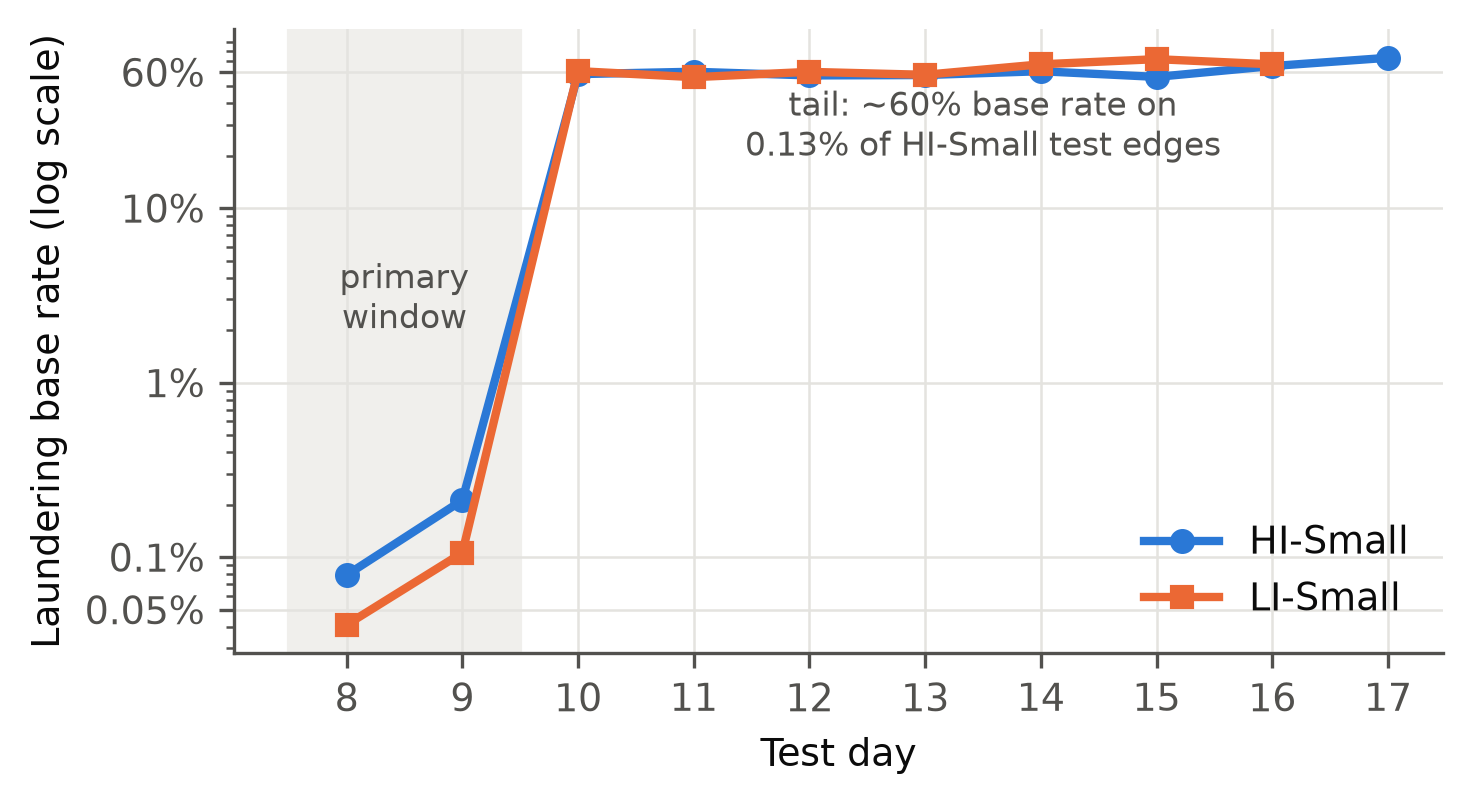
\includegraphics[width=0.62\textwidth]{fig_tail_base_rate.png}
\caption{Laundering base rate by test day in two AMLworld releases. After day 9 the
background traffic collapses and the base rate jumps by more than two orders of magnitude.}
% source: docs/paper/evaluation_protocol.md §4 (per-day base-rate table); figure built by paper_draft/make_figs.py
\label{fig:tail}
\end{figure}


Two consequences follow. A single-number test F1 on HI-Small is not comparable across papers
unless the window is stated: our detector's edge F1 is $0.495 \pm 0.027$ on days 8--9 and
0.596 on the whole split.
% source: results/tables/r1_edge_metrics.csv (primary_f1_minority_mean/std); r6_detector_swap.csv (edge_f1, gine_causal)
And the tail reaches ring-level results through the seed budget. A global 0.1\,\% score
quantile over the test split places only $463.0$ of its 864 seeds in the two clean days, so
any method that selects by a global quantile over this split operates in the clean window at
roughly half its nominal budget (Section~\ref{sec:results-swap} measures what recovering that
budget does).
% source: results/tables/v34_window_budget.json; docs/FINDINGS.md (dated note, window-matched seed budget)

\subsection{The day-0 warm-up}

Day 0 holds 34.3\,\% of HI-Small's training edges (34.4\,\% of LI-Small's) at roughly ten
times day 1's per-minute density. Trailing motif features count structures inside a time
window, so that density distorts them in both directions: cycle-shaped features are nonzero on
12.6\,\% of day-0 edges against about 2\,\% on every later day, while fan-in and fan-out
features are depressed (63\,\% against 89\,\%) because there is no history to look back on.
Both effects reproduce in LI-Small to within 0.3 percentage points.
% source: docs/FINDINGS.md (C8)
Day 0 is the simulation warming up, and anything trained across it is partly fitting that
warm-up.

How much this matters is release-specific. On HI-Medium, where day 0 is 48.8\,\% of training
edges at 0.27 times the later base rate, a detector trained across it reaches validation AP
0.3073; excluding day-0 \emph{labels} while keeping the day as message-passing history gives
0.4495 on half the supervised edges.
% source: docs/FINDINGS.md (C10)
The same exclusion does not help on HI-Small: with a gate fixed before training, seed-1
validation AP is 0.5455 against the reference detector's 0.5726, and the remaining seeds were
not run.
% source: docs/deep-analysis.md §9 — one seed; not yet recorded in docs/FINDINGS.md

\subsection{A global quantile can hand the seed budget to one day}

Every release ends its ordinary traffic with an elevated-volume day (1.36--1.57 times the
weekday norm). On HI-Medium, a single global 0.1\,\% quantile over the test split gives that
day 87.5\,\% of the seeds although it holds 16\,\% of the window's edges, because the
detector's scores are systematically higher there. On HI-Small the corresponding day takes
22.0--36.3\,\% of seeds across detector seeds against 75.8\,\% of the split's edges, so volume
alone does not explain the capture.
% source: docs/FINDINGS.md (C11); results/tables/v33_seed_by_day.csv
Budget allocation across days is a design choice and should be stated, not left to the score
distribution.

\subsection{Saturated scores break strict quantile cuts}
\label{sec:findings-saturation}

On one HI-Medium detector seed, 780{,}093 of 18.9\,M test scores are exactly 1.0. The 99.9\,\%
quantile is then 1.0 itself, and a strict ``score $>$ q'' rule selects no seeds at all.
Saturation grows with distance from training: 124 saturated edges on test day 6, 25{,}495 on
day 9 and 221{,}909 on day 15. Results from such a seed are an artefact of the cut, not a
measurement, and we exclude that seed from every HI-Medium number. The general point is that
a quantile rule is only defined once its tie handling is stated.
% source: docs/deep-analysis.md §7 (diagnosis 1: seed 3, 780,093 of 18.9 M scores at 1.0; 124 / 25,495 / 221,909 on days 6 / 9 / 15)

\subsection{The scope convention is worth five times the method}
\label{sec:findings-scope}

Figure~\ref{fig:scope} re-scores the same runs under four rules for what a truth ring's member
set is. Nothing is re-run and no parameter is re-chosen.

\begin{figure}[t]
\centering
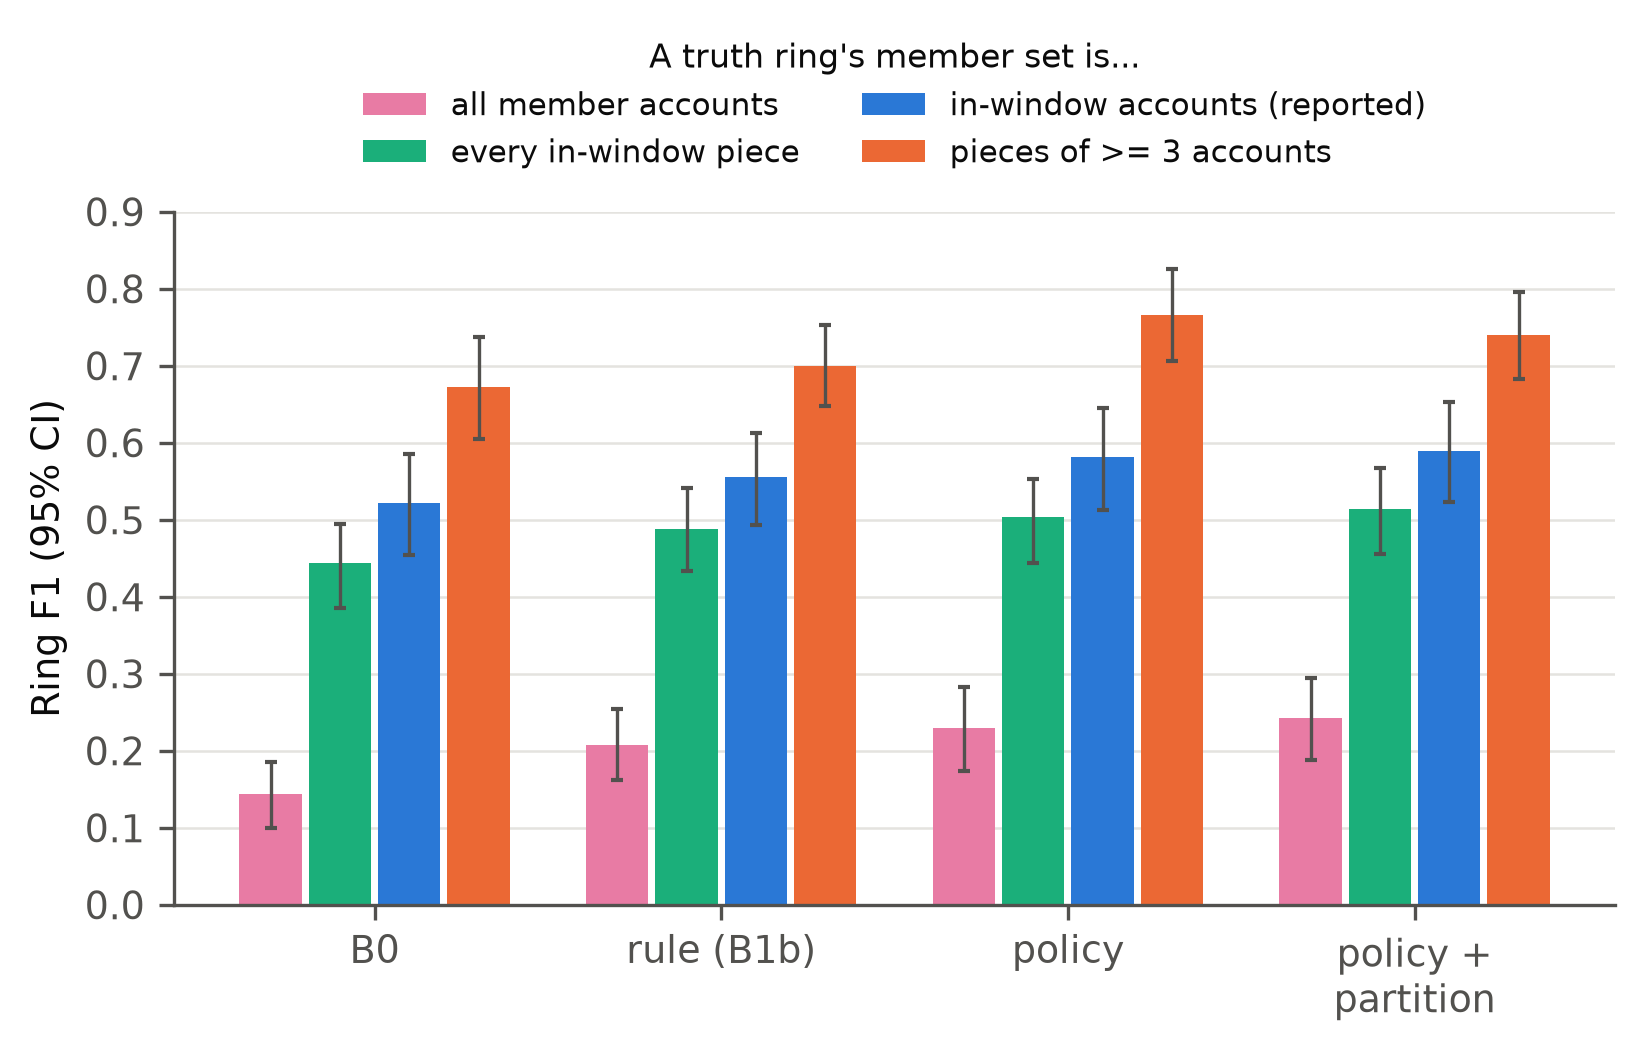
\includegraphics[width=0.78\textwidth]{fig_scope_conventions.png}
\caption{Ring-F1 of the same runs under four scope conventions (Multi-GINe detector, primary
window). The convention moves every method by far more than the methods differ from each
other.}
% source: results/tables/r14_scope_sensitivity.csv and v36_component_scope.csv; figure built by paper_draft/make_figs.py
\label{fig:scope}
\end{figure}

Counting all of a ring's accounts as members, not only those visible in the window, lowers
ring-F1 by 0.347--0.383 for every method and both GNN detectors (released repository). The in-scope ring count is unchanged at 174; only member sets grow, from a median
of 4 accounts to 11. For scale, the largest method effect in this paper is $+0.068$.
% source: results/tables/r14_scope_sensitivity.csv; docs/FINDINGS.md (C9)

Making targets smaller instead --- scoring each in-window connected piece of a ring as its own
target --- gives 254 targets; keeping only pieces of three or more accounts gives 108 targets
in 97 rings (released repository). The ordering
seeds $<$ rule $<$ policy $<$ policy-plus-partition is preserved under three of the four
conventions for both detectors. Under the fourth it changes in one place: the policy alone
overtakes policy-plus-partition (0.766 vs.\ 0.740). The swap was not tested for significance,
but the sign of the partition step flips, and it flips again on HI-Medium
(Section~\ref{sec:findings-hm}).
% source: results/tables/v36_component_scope.csv; docs/deep-analysis.md §4
Adding the community-detection baselines of Section~\ref{sec:results-baselines} shows what
re-ranking by convention looks like beyond that swap. Conventions re-rank methods that are
close, not methods that are clearly apart. The only other swaps between neighbours in the
ranking are seeds-plus-components against Louvain at resolution 0.5 (0.4436 vs.\ 0.4451 when
each in-window piece is a target; 0.6731 vs.\ 0.6738 with pieces of three or more accounts)
and the two weakest methods, Louvain at resolution 2 against CSGM, when all of a ring's
accounts count.
% source: results/tables/v40_external_baselines.json (bar_A adjacent_swaps); v40_external_baselines.csv (b0 / louvain_r0.5 component and component_ge3 ring_f1; louvain_r2 / csgm full_membership)

Neither extreme is right. Scoring against in-window accounts holds a method responsible only
for evidence it could have seen, and makes patterns severed by the split structurally
unmatchable. Scoring against all accounts keeps rings intact and penalises a perfect in-window
method for members it could not observe. A ring-level number is not interpretable without
knowing which rule produced it, and none of the group-level work we reviewed in
Section~\ref{sec:related} states one.
% source: docs/paper/evaluation_protocol.md §9

\subsection{A second release with ring-level evaluation: HI-Medium}
\label{sec:findings-hm}

HI-Medium has 2{,}187 in-scope rings in its primary window (test days 6--14), against
HI-Small's 174. We re-scored its existing ring outputs under the same protocol, with no new
training.
% source: results/tables/v41_hm_audit.json (observability.n_in_scope_rings; window); results/notes/p4_hm_audit.md
Under the earlier HI-Medium-trained detector, the direction of the scope effect reproduces but
not its size (ring-F1 lower by 0.038 to 0.073 across all eight cells, against a method effect of
0.092; tables in the released repository); observability reproduces (875 of 2{,}187 rings,
40.0\,\%, have no connected in-window piece of three or more accounts, against 44.3\,\% on
HI-Small); and the partition gain again falls with the Jaccard threshold (0.019 at 0.3 to 0.009
at 0.7), and under the three-account scope the policy alone again edges past
policy-plus-partition (0.2434 vs.\ 0.2430). Section~\ref{sec:results-hm} gives the transferred detector's rings on this release.
% source: results/tables/v41_hm_audit_scope.csv; v41_hm_audit.json (observability; verdicts.scope.global 0.0924); v41_hm_audit_threshold.csv

\subsection{A release without enough rings: LI-Small}

LI-Small was regenerated end to end (6{,}924{,}049 transactions, 705{,}907 accounts). The
preprocessing, splitting, scoping and windowing path runs unchanged, and the tail and day-0
artefacts reproduce. Its ring-level evaluation is under-powered --- 38 matchable rings in its
primary window against HI-Small's 114, below a stopping threshold fixed in advance --- so we
report no method numbers on it.
% source: docs/paper/evaluation_protocol.md §4 (LI-Small subsection)
      % 4 Benchmark audit
\section{Reference pipeline}
\label{sec:method}

The pipeline (Figure~\ref{fig:pipeline}) is deliberately conventional: a detector scores
edges, the highest-scoring edges seed candidate rings, and a ring layer grows and separates
them. It is the instrument for the measurements in Sections~\ref{sec:results}
and~\ref{sec:results-ceiling}, not the contribution.

\begin{figure}[t]
\centering
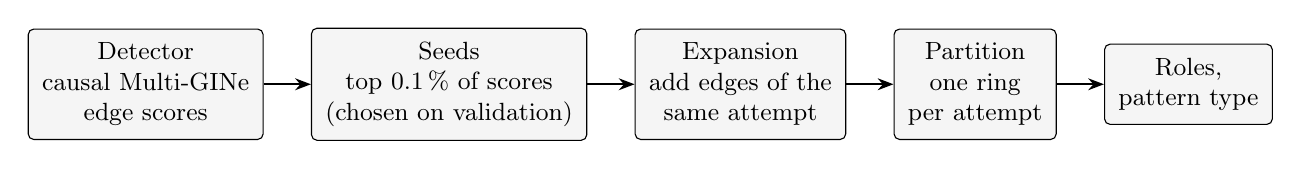
\begin{tikzpicture}[
  node distance=5mm and 6mm,
  stage/.style={draw, rounded corners=2pt, align=center, font=\small,
                minimum height=9mm, inner sep=5pt, fill=gray!8},
  arr/.style={-{Stealth[length=2mm]}, thick}
]
\node[stage] (l1) {Detector\\causal Multi-GINe\\edge scores};
\node[stage, right=of l1] (l2) {Seeds\\top 0.1\,\% of scores\\(chosen on validation)};
\node[stage, right=of l2] (l3a) {Expansion\\add edges of the\\same attempt};
\node[stage, right=of l3a] (l3b) {Partition\\one ring\\per attempt};
\node[stage, right=of l3b] (l3c) {Roles,\\pattern type};
\draw[arr] (l1) -- (l2);
\draw[arr] (l2) -- (l3a);
\draw[arr] (l3a) -- (l3b);
\draw[arr] (l3b) -- (l3c);
\end{tikzpicture}
\caption{The reference pipeline. ``B0'' denotes seeds grouped by connected components with no
further stage.}
% source: docs/report.md §3.2 (architecture, redrawn)
\label{fig:pipeline}
\end{figure}

\paragraph{Detector.}
A Multi-GINe edge classifier~\citep{egressy2024} with port numbering, time deltas, reverse
message passing, ego identifiers and subgraph-pattern edge features~\citep{blanusa2024},
trained with 5 seeds under batch-causal neighbour sampling (look-ahead within a batch of up to
1{,}800\,s; Section~\ref{sec:data}).
% source: docs/report.md §5.2
Causality matters here: a forward-looking variant of one cycle feature read edges after the
scored transaction and inflated its lift over the base rate by 12--16$\times$; made trailing,
the lift falls to 1.0--4.0$\times$ with primary-window edge F1 unchanged (0.495 vs.\ 0.494).
% source: docs/FINDINGS.md (C4)

\paragraph{Seeds.}
Seeds are the top $k^{*}=0.1\,\%$ of raw scores. The budget is fixed in advance for every detector
and seed; \texttt{min\_size} is chosen on validation ring-F1 (it is 3 throughout). As a sensitivity
analysis we also let validation choose $k^{*}$: it picks 0.1\,\% for every seed of Multi-GINe, but
0.05\,\% for two of five MEGA-GNN seeds, which lowers MEGA-GNN's full-pipeline ring-F1 from 0.602 to
0.510 (Table~\ref{tab:detector-swap}).
% source: configs/threshold_rule_k010.yaml; results/tables/r4_partition.csv (chosen_cells); results/tables/r6_detector_swap_sb2048_valpicked.csv (mega full 0.5098; seeds 4, 5 seed_frac_pct 0.05)

\paragraph{Expansion.}
A member edge below the seed cut --- a \emph{quiet member} --- never enters a baseline ring.
Expansion considers candidates that share an endpoint with an included edge within a
validation-chosen $\Delta t$ (up to two hops, capped at the 500 events nearest in time per
account to neutralise hub accounts).
% source: docs/EXPANSION.md §6.1
A LightGBM policy~\citep{ke2017} scores each candidate on 70 causal features: timing, money
conservation at the shared account, direction, reach to other seeds, trailing account state,
embedding similarity, detector-score quantile and trailing pattern counts.
% source: docs/EXPANSION.md §6.2
Its training data is cross-scored --- fold models trained on other days score each held-out
day --- so the policy never learns from in-sample detector scores; rows from day 0 are
dropped.
% source: docs/EXPANSION.md §6.3
The folds hold out days, not rings; Section~\ref{sec:limitations} reports the resulting leak
and its bound. We compare the policy with two rules: \emph{B1}, add every candidate sharing an
endpoint within $\Delta t$; and \emph{B1b}, the same with the candidate's score quantile above
0.99.
% source: docs/FINDINGS.md (B1)

\paragraph{Partition, roles and typing.}
A LightGBM affinity model scores pairs of ring edges that share an account, and
average-linkage clustering with a validation-chosen cut splits merged components. Each ring
then receives account roles from money-conservation rules and one of the eight pattern types
from a classifier over role counts, depth, cycle presence and size.
% source: docs/report.md §5.2

% Platform and explanation-layer paragraph moved to the released repository (cut rank 13).
        % 5 Reference pipeline
\section{Results with the reference pipeline}
\label{sec:results}

\subsection{Expansion recovers quiet members, and a two-line rule matches it}
\label{sec:results-expansion}

The detector reaches primary-window edge F1 $0.495 \pm 0.027$ and ROC-AUC 0.965.
% source: results/tables/r1_edge_metrics.csv (label=causal); docs/FINDINGS.md (A4)
Table~\ref{tab:ring-methods} gives the ring-level picture; Section~\ref{sec:results-baselines}
discusses the baselines in its upper block.

% Source: results/tables/r9_ring_ci.csv (rows b0, b1, b1b, proposed, average; window=primary) and
%         results/tables/v45_posthoc_ring_ci.csv (baselines and ring-folded rows; produced by
%         evaluation/r9_style_ci.py, which runs evaluation/step9_tables.py unmodified, so every
%         interval in this table is the same ring bootstrap: ring_stats.bootstrap_over_rings).
% Quiet-member recall is the point estimate from r9_quiet_members.csv / v45_posthoc_quiet_members.csv
% (FINDINGS convention, 2026-11-12), not the bootstrap mean in r9_ring_ci.csv.
\begin{table}[t]
\centering
\caption{Ring recovery on the primary window (174 truth rings, 5 seeds or runs,
in-window members, Jaccard $\ge 0.5$). Brackets: 95\,\% bootstrap intervals over truth rings,
seeds averaged inside each resample. Rows marked $^{*}$ use expansion-policy inputs folded by
ring (leak-free); the rows directly above them are the same methods with day-folded inputs, as
first reported. Rows marked $^{\S}$ are post hoc.}
\label{tab:ring-methods}
\small
\begin{tabular}{lccccc}
\toprule
Method & Ring prec. & Ring rec. & Ring F1 [95\,\% CI] & Member cov. & Quiet-member rec. \\
\midrule
CSGM~\citep{tian2025}$^{\dagger\S}$ & 0.321 & 0.048 & \ci{0.083}{0.047}{0.123} & 0.898 & --- \\ % source: v45_posthoc_ring_ci.csv (csgm, primary: 0.3208 / 0.0483 / 0.0834 [0.0474, 0.1227] / 0.8982)
Louvain, resolution 0.5$^{\S}$ & 0.795 & 0.382 & \ci{0.515}{0.428}{0.600} & 0.853 & 0.001 \\ % source: v45_posthoc_ring_ci.csv (louvain_r0.5); quiet v45_posthoc_quiet_members.csv (0.0013)
Louvain, resolution 1$^{\S}$ & 0.748 & 0.358 & \ci{0.483}{0.397}{0.563} & 0.834 & 0.009 \\ % source: v45_posthoc_ring_ci.csv (louvain_r1); quiet 0.0085
Louvain, resolution 2$^{\S}$ & 0.419 & 0.062 & \ci{0.107}{0.070}{0.148} & 0.655 & 0.002 \\ % source: v45_posthoc_ring_ci.csv (louvain_r2); quiet 0.0021
Label propagation$^{\S}$ & 0.785 & 0.377 & \ci{0.509}{0.421}{0.593} & 0.847 & 0.001 \\ % source: v45_posthoc_ring_ci.csv (lpa); quiet 0.0013
\midrule
Seeds + connected components & 0.814 & 0.384 & \ci{0.521}{0.429}{0.607} & 0.866 & 0.005 \\ % source: r9_ring_ci.csv (b0,primary)
Fixed expansion rule    & 0.171 & 0.162 & \ci{0.162}{0.118}{0.213} & 0.970 & 0.118 \\ % source: r9_ring_ci.csv (b1,primary); quiet: r9_quiet_members.csv (b1,primary,ALL = 0.1183)
Rule + score quantile  & 0.702 & 0.463 & \ci{0.555}{0.470}{0.632} & 0.943 & 0.223 \\ % source: r9_ring_ci.csv (b1b,primary); quiet: r9_quiet_members.csv (b1b,primary,ALL = 0.2229)
Learned expansion & 0.838 & 0.446 & \ci{0.582}{0.490}{0.668} & 0.942 & 0.209 \\ % source: r9_ring_ci.csv (proposed,primary); quiet: r9_quiet_members.csv (proposed,primary,ALL = 0.2092)
\quad ring-folded inputs$^{*\S}$ & 0.784 & 0.468 & \ci{0.585}{0.498}{0.670} & 0.960 & 0.251 \\ % source: v45_posthoc_ring_ci.csv (proposed_ringfold: 0.7835 / 0.4678 / 0.5848 [0.4980, 0.6699] / 0.9603); quiet 0.2510
\quad community step instead of components$^{\S}$ & 0.781 & 0.431 & \ci{0.555}{0.466}{0.641} & 0.897 & --- \\ % source: v45_posthoc_ring_ci.csv (lpa_on_expansion: 0.7806 / 0.4310 / 0.5550 [0.4663, 0.6408] / 0.8974)
\textbf{Full (expansion + partition)} & \textbf{0.818} & \textbf{0.461} & \textbf{\ci{0.589}{0.502}{0.675}} & \textbf{0.944} & \textbf{0.203} \\ % source: r4_partition.csv (average) / r9_ring_ci.csv (average,primary)
\quad ring-folded inputs$^{*\S}$ & 0.760 & 0.483 & \ci{0.589}{0.503}{0.672} & 0.960 & 0.243 \\ % source: v45_posthoc_ring_ci.csv (full_ringfold: 0.7597 / 0.4828 / 0.5893 [0.5034, 0.6722] / 0.9604); quiet 0.2425
\bottomrule
\multicolumn{6}{l}{\footnotesize $^{\dagger}$ External baseline, no detector; five runs over random two-institution splits of the accounts.}\\
\multicolumn{6}{l}{\footnotesize Community rows: the method run on the graph of the top-$k$\,\% flagged edges, $k$ chosen on validation per seed.}\\
\multicolumn{6}{l}{\footnotesize ``Community step instead of components'': label propagation on the learned expansion's subgraph, nothing tuned.}\\
\end{tabular}
\end{table}


Expansion from seeds recovers ring members the detector never fires on. With leak-free policy
inputs (Section~\ref{sec:limitations}), quiet-member recall rises from \ci{0.0052}{0.000}{0.015}
with seeds alone to \ci{0.251}{0.179}{0.344} with the learned policy, significant both on quiet
accounts per ring ($+0.432$ [$+0.301$, $+0.590$]) and on whole-ring matching ($+0.084$ [$+0.053$,
$+0.117$]), both $p_{\mathrm{Holm}}=0.0004$.
% source: results/notes/p2_ringfold.md (post hoc table); results/tables/v39_ringfold_quiet_members.csv; v39_ringfold_significance.csv (proposed_ringfold_vs_b0)
With the day-folded inputs we first reported and pre-registered, the recall was
\ci{0.2092}{0.142}{0.290}, with paired differences of $+0.359$ [$+0.236$, $+0.510$] and $+0.062$
[$+0.036$, $+0.092$], both $p_{\mathrm{Holm}}=0.0005$.
% source: results/tables/r9_quiet_members.csv (b0/proposed, primary, ALL); CIs r9_ring_ci.csv; r9_significance.csv (proposed_vs_b0)
It is the only one of the five pre-registered matched-ring comparisons to survive correction
(table in the released repository), and the result is stable across seed budgets: expansion
recovers 14--24\,\% of quiet members at every budget we tried
(released repository).
% source: docs/FINDINGS.md (section E)


\textbf{The learned policy is not what produces this recovery.} The rule B1b reaches
\ci{0.2229}{0.163}{0.299} quiet recall, indistinguishable from the policy on quiet accounts
($-0.024$ [$-0.084$, $+0.037$], $p_{\mathrm{Holm}}=1.00$) and on whole-ring matching
($p_{\mathrm{Holm}}=0.49$).
% source: docs/FINDINGS.md (B1, B2); r9_significance.csv (proposed_vs_b1b)
We ran this comparison on purpose, against our own method.

What the policy buys is the purity of what it adds. With leak-free policy inputs (cross-scores
folded by ring; Section~\ref{sec:limitations}) its added-member precision is 0.819 against the
rule's 0.518, a paired difference of $+0.301$ [$+0.235$, $+0.366$]; with the day-folded inputs we
first reported, the same comparison gave 0.926 and $+0.408$ [$+0.342$, $+0.479$],
$p_{\mathrm{Holm}}=0.0008$ (Figure~\ref{fig:quiet-precision}).
The leak-free comparison was run after the main results and is exploratory.
% source: results/tables/v39_ringfold_precision_paired.csv (proposed_ringfold_vs_b1b, added_member_precision: 0.8190 vs 0.5179, +0.3011 [+0.2349, +0.3657]); v35_precision_paired.csv (proposed_vs_b1b); paper/PREREG_AMENDMENT_2026-11-14.md §3
The matched-ring test cannot see this difference, which is why we test it with the
precision-aware paired bootstrap of Section~\ref{sec:data-stats}. The same test resolves the
gap between the pipeline on Multi-GINe scores and on GFP-XGBoost scores
($+0.139$ ring-F1 [$+0.083$, $+0.196$], $p_{\mathrm{Holm}}=0.0008$), which the matched-ring
test had scored at $p=0.807$: the weaker detector's pipeline matches about as many rings but
adds 2{,}419 edges at 26\,\% precision (day-folded inputs). The policy's ring-F1 gain over the
rule ($+0.027$) does not survive correction ($p_{\mathrm{Holm}}=0.093$); with leak-free inputs
it is $+0.030$ [$+0.010$, $+0.050$], outside the registered family.
% source: results/tables/v35_precision_paired.csv; docs/deep-analysis.md §2; v39_ringfold_precision_paired.csv (proposed_ringfold_vs_b1b, ring_f1: +0.0295 [+0.0101, +0.0501])

\begin{figure}[t]
\centering
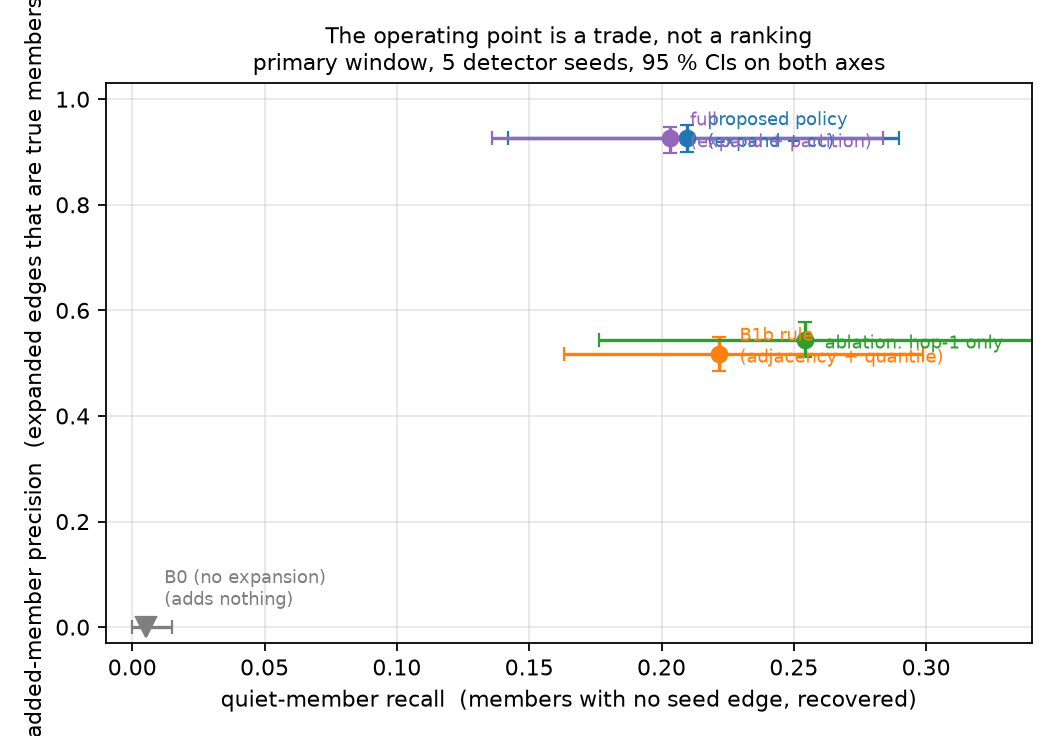
\includegraphics[width=0.55\textwidth]{r9_quiet_vs_precision.png}
\caption{Quiet-member recall against added-member precision (day-folded policy inputs, as first
reported; with leak-free inputs the policy's added-member precision is 0.819). The rule and the
policy recover similar shares of quiet members; they differ in how many wrong edges they add.}
% source: results/figures/r9_quiet_vs_precision.png (repository figure)
\label{fig:quiet-precision}
\end{figure}


\subsection{Community detection is not a stronger baseline than components}
\label{sec:results-baselines}

Replacing connected components with community detection on the same flagged-edge graph does
not help (Table~\ref{tab:ring-methods}, upper block; edge weight is the larger detector score
between two accounts, and the seed fraction is chosen on validation per seed). The best
community method by validation ring-F1, Louvain at resolution 0.5, reaches 0.515 on test,
against 0.521 for seeds and connected components ($-0.006$ [$-0.014$, $+0.000$],
$p_{\mathrm{Holm}}=0.072$) and 0.589 for the full pipeline ($-0.074$ [$-0.118$, $-0.035$],
$p_{\mathrm{Holm}}=0.0004$). Higher resolutions split rings apart (Louvain at resolution 2:
0.107). On the learned policy's expanded subgraph, label propagation in place of components
gives 0.555, below both components (0.582) and the average-linkage partition (0.589). CSGM,
collaborative scatter-gather mining~\citep{tian2025}, is designed for one pattern family and
uses no detector; over five random two-institution splits it reaches 0.083, with ring recall
0.048 over all eight pattern types. These comparisons were added after the main results.
% source: results/tables/v40_external_baselines.json (bar_B: louvain_r0.5 best by val; compare vs b0 / full, paired unit bootstrap 10,000 draws, Holm over two); v45_posthoc_ring_ci.csv (test_visible rows); results/notes/p3_baselines.md

\paragraph{An account-flagging method converted to rings.}
TAML~\citep{rico2026} flags illicit accounts per day and explains each with a signature. We trained it
on our split with its published settings (three seeds), took accounts above a validation-chosen
threshold on the two test days, and formed rings as connected pieces of its own graphs restricted
to those accounts. It reaches ring-F1 \ci{0.327}{0.254}{0.403} (precision 0.379, recall 0.287); a
per-day conversion gives 0.323. Three labels apply. Its features aggregate all ten days, test days
included; about 42\,\% of in-window ring transactions are absent from its graphs (247 of 585); and
so at most 63 of the 97 matchable rings can be formed. On those 63 its recall is 0.788. TAML solves
account flagging; converted to rings, it loses mainly through what its graphs omit. An exploratory
paired comparison with seeds-only MEGA-GenAgg rings ($+0.224$ [$+0.146$, $+0.304$]) is not a
superiority test.
% source: results/notes/p9_taml.md (2026-11-18 section); results/notes/final_numbers.md (TAML); experiments/R15_taml/scored_3seed_10k, paired_genagg_b0_vs_taml_joined

\subsection{Partition: not significant at 174 rings, resolved at 2{,}187}
\label{sec:results-partition}

On HI-Small the partition stage is not significant ($+0.015$ matched rate
[$-0.002$, $+0.036$], $p_{\mathrm{Holm}}=0.49$), nor is partitioning without expansion
($p_{\mathrm{Holm}}=0.23$). On HI-Medium, with 2{,}187 rings, an effect of the same size is
resolved: $+0.015$ [$+0.010$, $+0.020$], $p_{\mathrm{Holm}}=0.0003$
(Section~\ref{sec:results-hm}).
% source: results/tables/v3_closeout_p3.csv (global, full vs b2: mean_delta 0.01486, lo 0.00983, hi 0.01989, p_holm 0.0003)
Its pre-registered hypothesis --- that partitioning would allow a
looser seed budget --- was rejected: validation ring-F1 falls from 0.593 to 0.194 as the seed
fraction grows from 0.10\,\% to 0.50\,\%. A Louvain partition of the same expanded subgraph
leaves ring-F1 unchanged at 0.582.
% source: r9_significance.csv (full_vs_b2, cc_partition_vs_b0); docs/FINDINGS.md (B3, B4); results/tables/r4_partition.csv (b4)
On MEGA-GNN scores, where merged rings are commoner, the gain is the same size ($+0.017$)
and its interval excludes zero ($p_{\mathrm{Holm}} \approx 0.011$): over-merged rings fall
from 9.8 to 8.2 per seed there and stay at 5.2 on ours. The stage removes over-merges only
where they exist, and pays for recall with precision on both detectors.
% source: docs/FINDINGS.md (B3)
Its apparent benefit also depends on two evaluation choices: the recall gain is $+0.024$ at
Jaccard 0.3, $+0.015$ at 0.5 and $+0.001$ at 0.7, and it reverses when only connected pieces
of three or more accounts are scored (Section~\ref{sec:findings-scope}), on both releases.
On HI-Small we do not claim the partition step beyond neutral. Typing, held-out pattern types and time-to-detection are
in the released repository.
% source: docs/FINDINGS.md (B3; dated note, component-level scope)

\subsection{Transfer to a larger release}
\label{sec:results-hm}

On HI-Medium (test days 6--14, 2{,}187 rings), a detector trained only on HI-Small and applied
without retraining gives seeds-only ring-F1 $0.396 \pm 0.015$ over five seeds, against 0.090 for
an earlier HI-Medium-trained detector that differs in architecture and training data and has two
usable seeds (Table~\ref{tab:hm-transfer}; Section~\ref{sec:findings-saturation}). Paired over
the 2{,}187 rings the difference is $+0.306$ [$+0.286$, $+0.326$]; it comes from precision as
much as recall. We do not read this as transfer beating in-domain training: the comparison
changes the detector and its training data at once.
% source: results/notes/final_numbers.md (HI-Medium transfer); results/tables/hm_transfer_paired_addendum5.csv
Most of the gain is ranking, not budget allocation. The earlier detector put most of its global
budget on one day; allocating seeds per day lifts it to 0.148, while the transferred detector
stays at 0.387, so allocation explains at most about 0.06 of the 0.24 gap that remains.
% source: final_numbers.md (jump decomposition, five seeds); experiments_hi_medium/closeout_a15/log_seed{1,2}.json
The expansion policy and the partition were trained on HI-Medium with the earlier detector and
lack two of their inputs under transfer, so they are not evaluated here. With the earlier
detector, the release's 2{,}187 rings do resolve effects that 174 cannot: the partition gain is
$+0.015$ [$+0.010$, $+0.020$] (Section~\ref{sec:results-partition}).
% source: results/tables/v3_closeout_p3.csv (global, full vs b2)

% Source: results/notes/final_numbers.md (HI-Medium transfer section); results/tables/hm_transfer_closeout_seed{1..5}_ci.csv;
% results/tables/hm_transfer_paired_addendum5.csv (paired unit bootstrap over 2,187 rings, 10,000 draws, seeds averaged per draw).
\begin{table}[t]
\centering
\caption{Seeds-only rings (B0) on HI-Medium, test days 6--14, 2{,}187 rings, global 0.1\,\% budget,
in-window members, Jaccard $\ge 0.5$. The two detectors differ in architecture and training data.}
\label{tab:hm-transfer}
\small
\begin{tabular}{lcccc}
\toprule
Detector (seeds) & Precision & Recall & Ring F1 & Ring F1, per-day budget \
\midrule
Trained on HI-Small only, no retraining (5) & 0.444 & 0.357 & $0.396 \pm 0.015$ & $0.387 \pm 0.015$ \
Trained on HI-Medium, earlier detector (2) & 0.126 & 0.074 & 0.090 & 0.148 \
Paired difference & $+0.318$ & $+0.283$ & $+0.306$ [$0.286$, $0.326$] & -- \
\bottomrule
\end{tabular}
\end{table}


\subsection{Edge F1 is not a proxy for ring recovery}
\label{sec:results-swap}

We re-ran the ring layer on other detectors at the same fixed 0.1\,\% seed budget, re-choosing
every other downstream parameter on validation per detector and seed (Figure~\ref{fig:edge-ring}, Table~\ref{tab:detector-swap}).
Our MEGA-GNN reproduction reaches $0.6856 \pm 0.0447$ test edge F1, against the
$0.7083 \pm 0.0218$ its authors report for the same configuration; the gap is attributable to
batch-causal sampling (Section~\ref{sec:data}), which their setup does not use\footnote{All MEGA-GNN scores in this paper are produced with a scoring batch of 2048 transactions. The released models were originally scored at 8192, which gives test edge F1 $0.6893 \pm 0.0396$ against $0.6856 \pm 0.0447$ at 2048; per seed, 2048 minus 8192 is $-0.0126$, $-0.0029$, $-0.0013$, $+0.0049$ and $-0.0069$. The causal neighbour sampler cuts batches by size or by 30 minutes of seed time, whichever comes first, so a larger scoring batch lets a transaction see later transactions of the same batch (median look-ahead 180\,s at 2048, 600\,s at 8192). The validation-to-test gap per seed is in the released repository.}.
% source: results/notes/p7_genagg.md (batch-2048 per-seed table, look-ahead); results/notes/p7_batch_span.json
% source: docs/paper/generalisation.md §1

\begin{figure}[t]
\centering
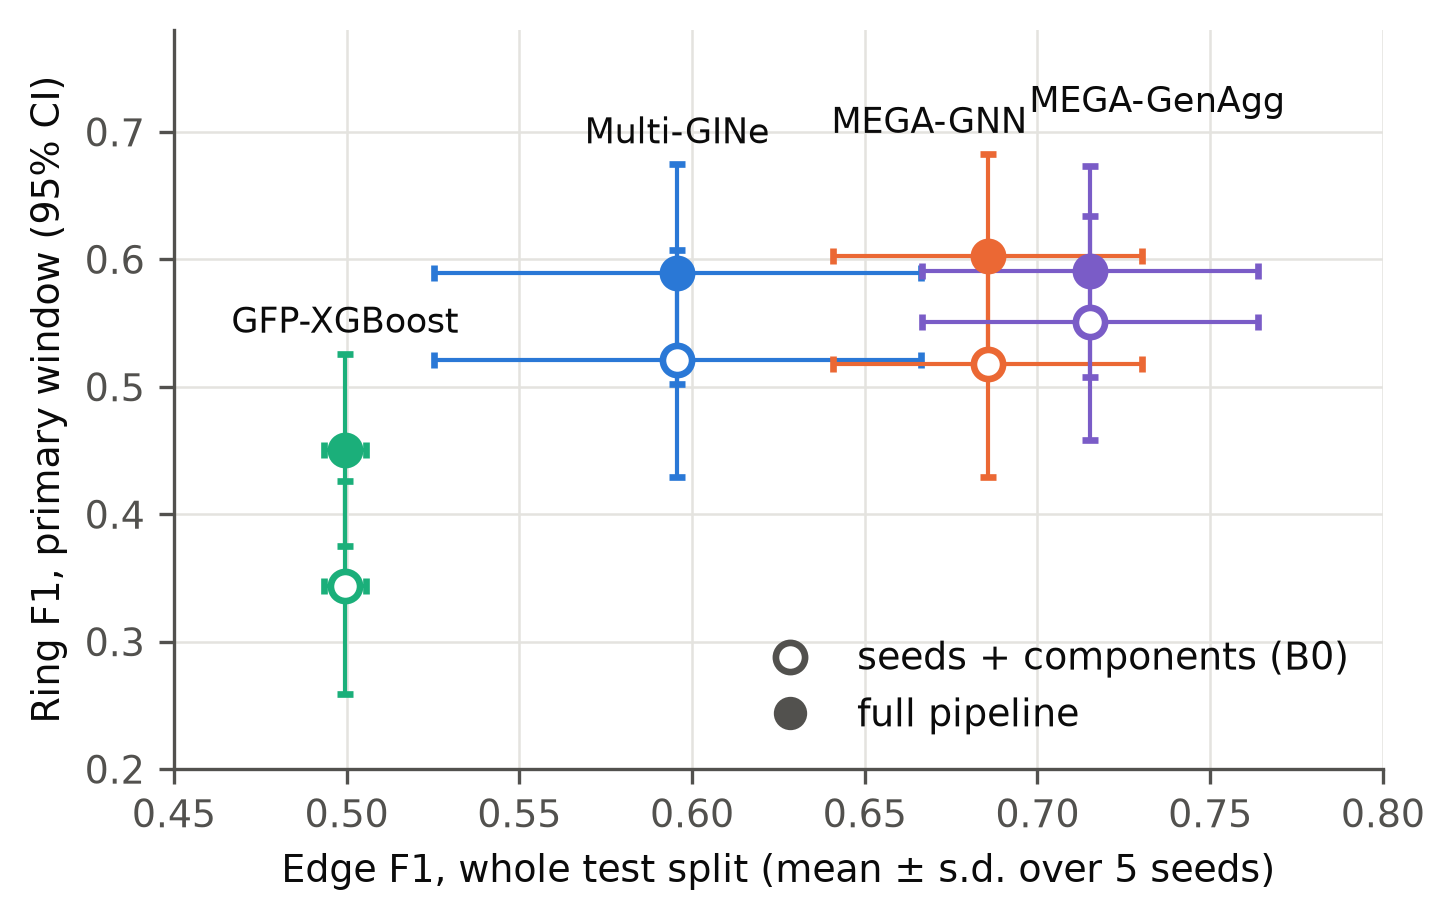
\includegraphics[width=0.62\textwidth]{fig_edge_vs_ring_sb2048.png}
\caption{Edge F1 against ring F1 for four detectors (scoring batch 2048). From Multi-GINe to
MEGA-GenAgg, 12 points of edge F1 leave seeds-only ring F1 within 0.03; below Multi-GINe, ring
F1 falls with edge F1.}
% source: results/tables/r6_detector_swap_sb2048.csv, r6_genagg_5seed.csv; figure built by evaluation/make_figs_sb2048.py
\label{fig:edge-ring}
\end{figure}

% Source: results/tables/r6_detector_swap.csv
\begin{table}[t]
\centering
\caption{The same ring layer on three detectors, every downstream parameter
re-chosen on validation per detector per seed. Edge F1 is on the whole test split (mean $\pm$
std over 5 seeds); ring numbers are on the primary window with bootstrap CIs. Added-member precision here was measured with day-folded expansion-policy inputs; with leak-free (ring-folded) inputs the reference full pipeline's value is 0.817 (Table~\ref{tab:precision-paired}).}
% source (leak-free value): results/tables/v45_ringfold_full_precision_paired.csv (full_ringfold, added_member_precision 0.8174)
\label{tab:detector-swap}
\small
\begin{tabular}{lccccc}
\toprule
Detector & Edge F1 & Ring F1, B0 & Ring F1, full & Quiet rec., full & Added prec., full \\
\midrule
GFP-XGBoost & $0.500 \pm 0.006$ & \ci{0.343}{0.259}{0.426} & \ci{0.451}{0.375}{0.526} & 0.267 & 0.260 \\ % source: r6_detector_swap.csv (gfpxgb rows)
Multi-GINe (shipped) & $0.596 \pm 0.071$ & \ci{0.521}{0.429}{0.607} & \ci{0.589}{0.502}{0.675} & 0.203 & 0.926 \\ % source: r6_detector_swap.csv (gine_causal rows)
MEGA-GNN & $0.689 \pm 0.040$ & \ci{0.521}{0.432}{0.609} & \ci{0.607}{0.521}{0.688} & 0.242 & 0.932 \\ % source: r6_detector_swap.csv (mega rows)
\bottomrule
\end{tabular}
\end{table}


MEGA-GNN outscores Multi-GINe by 9.0 points of edge F1 and produces the same baseline rings
(ring-F1 0.518 vs.\ 0.521) at the fixed budget. MEGA-GenAgg, 12.0 points above Multi-GINe
($0.715 \pm 0.049$), gives seeds-only ring-F1 0.551, a paired difference of $+0.030$
[$-0.011$, $+0.072$]; with the full pipeline the difference is $+0.002$ [$-0.030$, $+0.034$].
% source: results/notes/final_numbers.md (detector-swap rows); results/tables/r6_genagg_paired.csv (exploratory family, Holm over 4) When validation chooses the budget instead,
two MEGA-GNN seeds pick 0.05\,\% and its rings fall behind (Section~\ref{sec:method}).
% source: results/tables/r6_detector_swap_sb2048.csv; docs/FINDINGS.md (C6)
This is not the detectors agreeing. MEGA-GNN's and Multi-GINe's seed sets overlap at Jaccard
0.409, yet they reach 127.4 and 129.6 of the 174 truth rings. What binds at this operating point is how many rings a
0.1\,\% quantile can reach, not the ranking that fills it. The relation is a ceiling, not
independence: the weaker GFP-XGBoost, 9.6 edge points below, loses 17.7 ring points.
% source: docs/FINDINGS.md (C6)
The claim is conditional on this budget, these graph neural detectors (edge F1 0.60 to 0.72)
and this dataset; below that range the detector still decides recovery
(Section~\ref{sec:results-hm}).
% source: results/tables/r6_seed_overlap_sb2048.csv

\paragraph{Can the budget be spent better?}
Each GNN detector touches about 74\,\% of truth rings and their touched sets overlap at
70.6\,\%, so their union reaches 150.8 of 174 --- but that is two full budgets. At the same
budget, a best-rank ensemble of the two reaches 133.6, about a fifth of the gap, because 484
of the 864 selected edges are in both detectors' top 0.1\,\%. A per-account budget reaches
fewer (116.2). At an equal budget neither reallocation changes baseline ring-F1 beyond seed
noise (0.521 / 0.515 / 0.519), and under the full pipeline the ensemble's gain
($+0.021 \pm 0.038$) is inside seed spread.
% source: docs/FINDINGS.md (C7, B14 with its dated correction); results/tables/v37_realloc_full.csv

\paragraph{The effective test budget is about half the nominal one.}
Only 463 of 864 seeds land in the primary window (Section~\ref{sec:findings-tail}). Spending the
whole budget inside it reaches more rings (148.2 against 129.6) but lowers ring-F1 from 0.589 to
0.546 on every seed, so the reported ring-F1 is not depressed by the budget lost to the tail
(table in the released repository).
% source: results/tables/v34_window_budget.json; docs/deep-analysis.md §1

\section{Where ring recovery stops}
\label{sec:results-ceiling}

Figure~\ref{fig:decomposition} accounts for all 174 truth rings. With the full pipeline on
Multi-GINe, the detector we use for loss counts throughout, 80.2 are matched per seed, 48.6 have fewer than three visible members and
go unmatched, 33.2 are untouched by any seed or expanded edge, 5.2 are merged with a
neighbour and 6.8 are recovered only in part. Achieved ring recall is
\ci{0.461}{0.393}{0.529}.
% source: docs/FINDINGS.md (B11); results/tables/r6_detector_swap.csv; r9_ring_ci.csv (average, primary, ring_recall)

\begin{figure}[t]
\centering
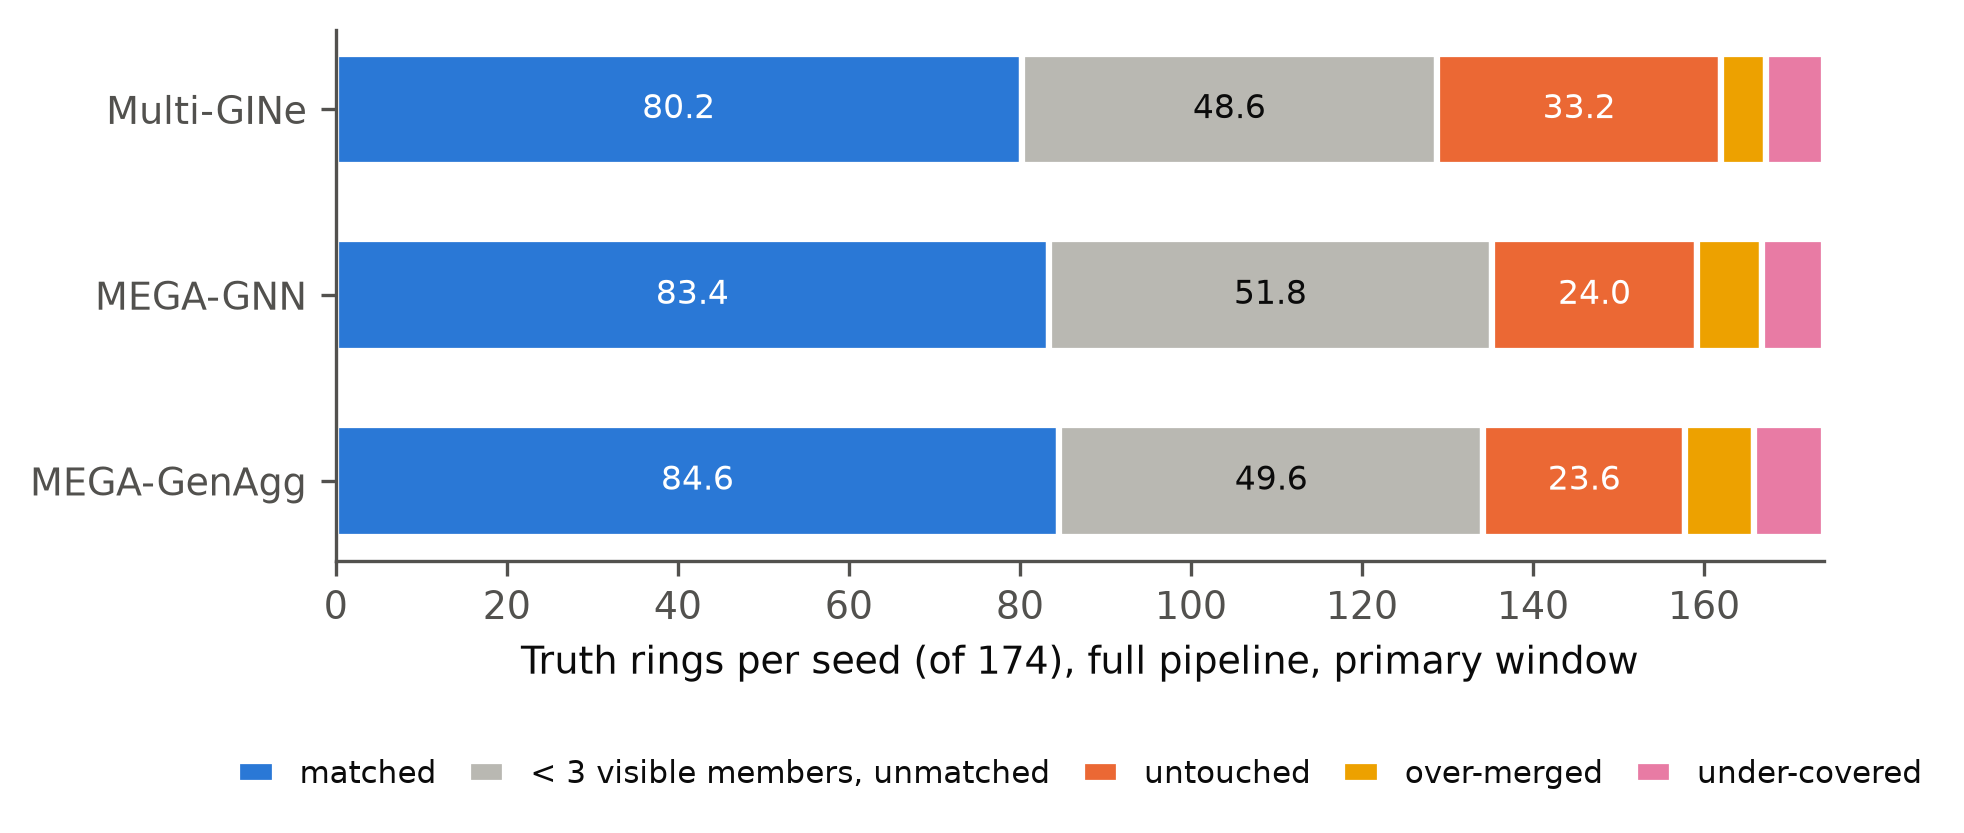
\includegraphics[width=0.9\textwidth]{fig_ring_decomposition_sb2048.png}
\caption{What happens to the 174 primary-window truth rings (per seed, full pipeline). The text
uses the Multi-GINe bars; the other detectors are shown for comparison only.}
% source: docs/FINDINGS.md (B11); figure built by paper_draft/make_figs.py
\label{fig:decomposition}
\end{figure}

\paragraph{Small rings are not a hard ceiling.}
60 of the 174 rings have fewer than three visible members, yet the pipeline matches
$11.4 \pm 2.3$ of them per seed, most at Jaccard 1.0, because \texttt{min\_size} applies to
the unrestricted prediction while matching uses the window-restricted one. The share of rings
with three or more visible members (114 of 174) is a reference level, not a bound.
% source: docs/FINDINGS.md (B7, B9, as corrected)

\paragraph{Partially recovered rings are clean, short fragments of long patterns.}
In every one of the 34 partially recovered instances the prediction contains no wrong
account, and it holds a median 3 of the ring's 14 members. Thirteen distinct rings produce all
34 instances, half of them STACK.
% source: docs/FINDINGS.md (B12); results/tables/r_under_covered.csv

\paragraph{Most of what is missing is disconnected inside the window.}
For each partially recovered ring we measured the distance from the recovered fragment to the
ring's missing member edges, through the ring itself, inside the primary window. 176 of 216
missing edges (81.5\,\%) lie in a piece with no path to the fragment at all --- all 140 for
STACK, all 24 for BIPARTITE --- and 85.6\,\% were never generated as candidates. The exception
is GATHER-SCATTER, whose 31 missing edges sit one hop away and were declined by the policy; an
oracle admitting exactly those edges completes all 8 instances, about 1.6 rings per seed,
whereas lowering the policy's floor to reach them costs more precision than validation
accepts.
% source: docs/FINDINGS.md (B13, B15); results/tables/r_in_window_connectivity.csv
Widening the window to all ten test days reduces disconnection to 52.3\,\% and removes it for
CYCLE and RANDOM, but STACK stays at 100\,\% (237 of 237): its chains are severed by the
train/validation/test split itself. Traversing the full 18-day graph backwards under the
expansion's own rules reaches none of the 140 missing STACK edges at two or three hops, and a
permutation null reaches none of 216.
% source: docs/FINDINGS.md (B13, B16); results/tables/r_historical_bridge.csv
A supervised-contrastive head~\citep{khosla2020} trained on the frozen detector embeddings to
recognise ring identity does not reconnect the pieces either: same-ring separability across
components rises only from AUC 0.552 to 0.618, against a bar of 0.75 fixed in advance.
% source: docs/deep-analysis.md §10 — registered follow-up; not yet recorded in docs/FINDINGS.md

\paragraph{Observability, counted directly.}
77 of the 174 rings (44\,\%) have no connected in-window piece of three or more accounts. 60
of them are the small rings above; the other 17 have enough visible members, split across
pieces that are each too small, and are scored as ordinary misses. On the 97 rings that do
have a matchable piece, the pipeline recovers 70.6\,\% of the pieces, and STACK recall rises
from 0.036 to 0.493.
% source: docs/FINDINGS.md (dated note, component-level scope); results/tables/v36_component_scope.csv

Taken together, the binding constraint is neither seed allocation nor policy thresholds. It is
how much of a ring is observable and connected inside the evaluation window --- a property of
the split and the scope rule that is easy to mistake for a property of the method.

\subsection{What did not help}
\label{sec:results-negative}
We made nine attempts to spend the seed budget better or to reassemble rings after the
detector, all at the fixed 0.1\,\% budget (primary window, test-visible truth, Jaccard 0.5, five
seeds, Multi-GINe scores): five were read on test and four stopped at their validation gate. None
raised ring-F1. The reference is the shipped full pipeline, or for the verifier, motif search and
flow-following the leak-free one; both score 0.589 on test.
% source: results/notes/recovery_attempts.md (list confirmed against q_track, m_track, recovery_ensemble, recovery_history, FINDINGS B14)
\begin{itemize}
\item \emph{Best-rank seed fusion} of two detectors (test): $+0.021 \pm 0.038$, inside seed spread.
\item \emph{Per-account seed budget} (test): fewer rings reached (116.2 against 129.6) and lower ring-F1.
% source: docs/FINDINGS.md (B14); results/tables/v37_realloc_full.csv
\item \emph{Account-level seeding} (test): $-0.138$ [$-0.184$, $-0.093$].
% source: results/notes/q_track.md (Q2); results/tables/q_family_holm.csv
\item \emph{Over-generate at 0.2\,\% and verify} (test): $+0.004$ [$-0.041$, $+0.046$]; precision up
$0.098$, recall down $0.029$.
% source: results/tables/m1_primary.json
\item \emph{History-reserved seeds} for accounts with labelled history (test): $+0.003$ [$-0.022$, $+0.030$].
% source: results/notes/recovery_history.md (B2); results/tables/b2_test_r25_both_paired.csv
\item \emph{Undersized-group rescue} (validation): no relaxed cell beat the shipped one.
% source: results/notes/q_track.md (Q6)
\item \emph{Temporal motif search} and \emph{flow-following} (validation): both gates failed (0.569 against 0.585).
% source: results/tables/m2_gate.json, m3_gate.json
\item \emph{Rank-averaged detector ensemble} as the seed source (validation): 0.575 against 0.593.
% source: results/notes/recovery_ensemble.md
\end{itemize}
The loss breakdown says why (Multi-GINe full pipeline, per seed; the one detector we use for loss
buckets throughout). Of 174 rings, 77 have no in-window piece of three or more accounts (11.4 of
them still matched), 11.0 are matchable but touched by no seed, 14.4 are recovered too thinly, and
merges (1.0) and splits (1.8) account for little; 68.8 are matched. Of the 93.8 unmatched rings,
65.6 are in the first group. Reassembly can only rearrange what the seeds already reach.
% source: results/notes/q_track.md (Q0 table); results/tables/q0_buckets.csv
       % 6 Results; 7 Where recovery stops
\section{Recommendations for reporting ring-level AML results}
\label{sec:recommendations}

Each recommendation below follows from a measurement in this paper.

\begin{enumerate}
\item \textbf{State the scope rule.} Say which accounts count as a ring's members when the
  ring crosses the evaluation window. The choice is worth 0.35--0.38 ring-F1 on HI-Small and
  0.04--0.07 on HI-Medium (Sections~\ref{sec:findings-scope} and~\ref{sec:findings-hm}).
% source: results/tables/r14_scope_sensitivity.csv; results/tables/v41_hm_audit_scope.csv
\item \textbf{State the split and the window, and report the tail separately.} On AMLworld's
  day split, do not average over days 10--17 (Section~\ref{sec:findings-tail}).
\item \textbf{State how a selection budget is allocated across days.} A global quantile can
  give one day most of the budget, and on this split gives the clean window about half
  (Sections~\ref{sec:findings-tail} and~\ref{sec:results-swap}).
\item \textbf{State the tie-handling rule of any quantile cut.} When many scores are tied at
  the cut, ``score $>$ q'' and ``score $\ge$ q'' select very different sets; on one saturated
  HI-Medium detector the strict rule selects no seeds at all
  (Section~\ref{sec:findings-saturation}).
\item \textbf{Sweep the matching threshold.} Report the gain at a stricter threshold wherever
  it is reported at 0.5; a gain that vanishes at 0.7 is fragmentation
  (Section~\ref{sec:results-partition}).
\item \textbf{Resample rings, not edges, and test precision.} Matched-ring tests cannot see
  false rings; pair them with a test that can (Section~\ref{sec:data-stats}).
\item \textbf{Never quote recovered-member recall without the precision of what was added.}
  The weakest detector in our comparison posts the highest quiet-member recall, at 26\,\%
  added-member precision (Table~\ref{tab:detector-swap}).
\item \textbf{Report how many targets are observable.} Count the rings that have a connected,
  matchable piece in the window, and report recall on those beside recall on all
  (Section~\ref{sec:results-ceiling}).
\item \textbf{Do not use edge F1 as evidence of better group recovery.} Run the group-level
  evaluation (Section~\ref{sec:results-swap}).
\item \textbf{Include a rule baseline.} A two-line rule matched our learned component's recall
  (Section~\ref{sec:results-expansion}).
\end{enumerate}

\section{Limitations}
\label{sec:limitations}

\paragraph{One generator family.}
Everything here is AMLworld. The tail and warm-up are reproduced on LI-Small; on HI-Medium the
warm-up, the budget capture, the share of unobservable rings, the threshold dependence of the
partition gain and the direction (not the size) of the scope effect reproduce, from a detector
that missed its adequacy bar and two usable seeds; the transferred detector's seeds-only rings
are the only HI-Medium method numbers we report under transfer. All three releases come from one simulator;
nothing establishes how the findings carry to other generators or to real transaction data. Method
comparisons rest on 174 truth rings and 5 detector seeds, and only one of five pre-registered
comparisons survives correction at that power.
% source: docs/FINDINGS.md (A6); docs/paper/generalisation.md §3

\paragraph{External baselines.}
We score two external group-level methods (CSGM over five random two-institution splits; TAML,
three seeds, converted to rings) and two families of community detection under the protocol.
TAML is scored with protocol differences we could not remove: its features aggregate all ten
days, and its graphs omit about 42\,\% of in-window ring transactions. Leiden was planned but not
run, and \citet{chai2023} was not run.
% source: results/tables/v40_external_baselines.json (runs, notes); results/notes/p3_baselines.md

\paragraph{The edge-versus-ring claim is conditional.}
It is measured at one seed budget, across three graph neural detectors from edge F1 0.596 to
0.715, on one dataset. Below that range it does not hold (GFP-XGBoost, HI-Medium), and detectors
above it were not tested.

\paragraph{A ring-level leak in the expansion policy's training data.}
The policy's cross-scored inputs hold out a day per fold, but rings span days, so a fold model
is supervised on some edges of a ring and then scores that ring's held-out-day edges. Between
65.0\,\% and 92.4\,\% of each fold's held-out rings are affected. The measured effect is small
--- the gap in ROC-AUC between affected and unaffected ring edges ranges from $-0.008$ to
$+0.036$ across folds, and unaffected rings are still scored at AUC 0.958--0.996 --- and the
leak touches training inputs only: test scores come from a detector trained on the train
split alone. Removing the affected feature group changes primary-window ring-F1 by 0.008,
which bounds what a leak-free version could change on HI-Small; on HI-Medium the same ablation
moves validation ring-F1 by 0.026 in the opposite direction, so the bound does not transfer
between releases.
% source: docs/FINDINGS.md (B17); results/tables/v33_ring_fold_leakage.csv, v33_leak_inflation.csv, v33_policy_ablations.csv
We re-ran the policy with its inputs folded by ring, so that no fold model sees any edge of a
ring it scores. The registered check on the mean ring-F1 difference passed ($+0.0028$, inside
$\pm 0.008$), but the paired interval, $[-0.0137, +0.0211]$ ($p=0.77$), is too wide to call the
two equivalent, so on ring-F1 the comparison is inconclusive. The leak did inflate precision:
with leak-free inputs, ring precision falls from 0.838 to 0.784 ($-0.055$ [$-0.089$, $-0.027$])
and added-member precision from 0.926 to 0.819, while ring recall rises by 0.022. The full
pipeline behaves the same way: ring-F1 0.589 with either input ($-0.000$ [$-0.017$, $+0.019$]),
added-member precision 0.926 against 0.817. Where this paper reports added-member or ring
precision, the leak-free value is given first. These re-runs were added after the main results
and are exploratory.
% source: docs/deep-analysis.md §8 (verdict) and §15; results/tables/v39_ringfold_report.csv (paired: ring_f1, ring_precision, ring_recall, added_member_precision); v45_ringfold_full_precision_paired.csv (full_ringfold_vs_full); v45_posthoc_ring_ci.csv; paper/PREREG_AMENDMENT_2026-11-14.md

\paragraph{Analyses added after the main results.}
The precision-aware paired test, the window-matched budget, the component-level scope and the
reallocation analysis were run on a test window that had already been examined many times.
Their designs and bars were written down before each was run, but they are sensitivity
analyses, not confirmatory tests. None changes a reported point estimate.
% source: docs/FINDINGS.md (section G preamble); docs/deep-analysis.md (header and caveats)

\paragraph{Published-number comparison.}
The only published figure we compare against is MEGA-GNN's edge F1
(Section~\ref{sec:results-swap}).

\paragraph{Evaluation defects we found.}
Each changed a number we had reported, and each is corrected here: bootstrap resamples that
collapsed repeated rings (intervals about a quarter too narrow); matcher ties broken by file
order; detector scores that depend on the scoring batch through batch-level causal sampling, and
the look-ahead that sampling allows (Section~\ref{sec:data}); a ring-level leak through
day-folded policy inputs (above); a global quantile that hands the seed budget to one day; and
saturated scores that leave a strict quantile cut empty (Section~\ref{sec:findings}).
% source: results/notes/interval_consistency.md; matcher_tiebreak.md; p7_genagg.md (scoring batch, look-ahead); FINDINGS B17, C11; findings saturation

\section{Conclusion}
\label{sec:conclusion}

When the unit of evaluation is the laundering attempt, the numbers AMLworld produces are
governed first by choices that papers rarely state and only then by the method. The scope rule
is worth 0.35--0.38 ring-F1. The standard split's tail inflates edge metrics and halves the
effective seed budget in the two days that carry ordinary traffic. And 44\,\% of in-scope
rings cannot be matched as connected objects by any method, because the split and the window
sever them.
% source: docs/FINDINGS.md (C9, C1 and dated notes on the window-matched budget and component-level scope)

Within those limits, detector quality decides ring recovery only up to a point. On HI-Small,
three graph neural detectors from edge F1 0.596 to 0.715 give seeds-only ring-F1 0.518 to 0.551,
and nine attempts to spend the budget better or reassemble rings after the detector leave
ring-F1 flat; most remaining losses are rings with too few visible members. Below that range the
detector still matters: on HI-Medium a detector trained only on HI-Small, applied without
retraining, gives $0.396 \pm 0.015$ against 0.090 for an earlier in-domain detector that differs
in architecture and training data, mostly through ranking. TAML, converted to rings, reaches
0.327 and loses mainly through what its graphs omit.
% source: results/notes/final_numbers.md (detector swap, HI-Medium transfer, TAML); results/notes/recovery_attempts.md

The practical consequence is for how group-level AML results are reported. A ring-level number
is interpretable only with its scope rule, split, window, budget allocation and matching
threshold attached, and edge F1 is not evidence about it. We release the protocol, the tables
behind every number in this paper, and the code.


\section*{Acknowledgements}
% source: CONTRIBUTORS.md
Ruhani Kumar built the explanation layer and the Elliptic baselines, and found the evaluation
defect in ring typing that Appendix~\ref{app:corrections} records; Kashish Mittal built the
multi-tenant platform; Lakshmishree produced the dashboard mockup.
% source: CONTRIBUTORS.md; docs/FINDINGS.md (typing correction, 2026-10-22)

\bibliographystyle{plainnat}
\bibliography{refs}

\appendix
\section{Reproducibility}
\label{app:repro}

All runs: Intel Xeon W-2295 (18C/36T), 128\,GB RAM, NVIDIA RTX A5000 (24\,GB), Windows 11,
Python 3.12, PyTorch 2.5.1+cu121, PyG 2.8.0.
% source: README.md (Hardware)
Every reported number recomputes from a run's stored metrics; an audit script re-derives 18
headline rows mechanically (18 traceable, 0 mismatched), and a frozen-numbers file pins every
headline to its source with a failing test on change.
% source: README.md; docs/REPRODUCE.md §13 (row 6); results/FROZEN.json

\paragraph{Data integrity.}
Edge identifiers are row positions after a stable sort on timestamps, so a manifest check pins
the inputs:
% source: docs/REPRODUCE.md §0

\begin{center}\small
\begin{tabular}{lll}
\toprule
File & SHA-256 (first 16) & Bytes \\
\midrule
\texttt{HI-Small\_Trans.csv} & \texttt{b19d39f515523373} & 475{,}664{,}283 \\ % source: docs/REPRODUCE.md §0
\texttt{HI-Small\_accounts.csv} & \texttt{786808526e33cfc4} & 34{,}053{,}187 \\ % source: docs/REPRODUCE.md §0
\texttt{HI-Small\_Patterns.txt} & \texttt{2c546b5ce6009e73} & 323{,}844 \\ % source: docs/REPRODUCE.md §0
\texttt{formatted\_transactions.csv} & \texttt{3b9678458eeece7e} & 266{,}605{,}148 \\ % source: docs/REPRODUCE.md §0
\bottomrule
\end{tabular}
\end{center}

\paragraph{End-to-end check.}
With nothing retrained, the data manifest passes, the research test suite passes 258 tests,
and the ring-building command regenerates the released rings byte-identically (108 rings in
62\,s).
% source: docs/REPRODUCE.md §13 (rows 1, 2a, 7)
Measured training times: detector about 15\,h for 5 seeds; cross-scoring about 8\,h; MEGA-GNN
about 18\,h; statistics about 45\,min.
% source: docs/REPRODUCE.md §2, §4, §7, §8

\section{Additional results}
\label{app:tables}

\paragraph{Scope conventions.}
Tables~\ref{tab:scope} and~\ref{tab:component-scope} give the numbers behind
Figure~\ref{fig:scope}.

% Source: results/tables/r14_scope_sensitivity.csv, as summarised in
%         docs/paper/evaluation_protocol.md §9 (same shipped runs re-scored; no model re-run)
\begin{table}[t]
\centering
\caption{The scope convention moves ring-F1 about five times more than the entire method does.
The same shipped runs re-scored under \texttt{full\_membership} (a ring's member set is all its
accounts) against the reported \texttt{test\_visible}; the method ordering survives under both.}
\label{tab:scope}
\small
\begin{tabular}{lccc}
\toprule
Detector / method & \texttt{test\_visible} (reported) & \texttt{full\_membership} & Gap \\
\midrule
GINe B0 & 0.5213 & 0.1437 & $-0.378$ \\ % source: r14_scope_sensitivity.csv (gine_causal b0 rows, ring_f1)
GINe B1b & 0.5553 & 0.2073 & $-0.348$ \\ % source: r14_scope_sensitivity.csv (gine_causal b1b rows)
GINe proposed & 0.5819 & 0.2297 & $-0.352$ \\ % source: r14_scope_sensitivity.csv (gine_causal proposed rows)
GINe full & 0.5894 & 0.2428 & $-0.347$ \\ % source: r14_scope_sensitivity.csv (gine_causal full rows)
MEGA B0 & 0.5208 & 0.1595 & $-0.361$ \\ % source: r14_scope_sensitivity.csv (mega b0 rows)
MEGA full & 0.6074 & 0.2252 & $-0.382$ \\ % source: r14_scope_sensitivity.csv (mega full rows)
\bottomrule
\end{tabular}
\end{table}

% Source: results/tables/v36_component_scope_wci.csv (v36_component_scope.csv re-scored with the
%         weighted ring bootstrap by evaluation/rescore_weighted_intervals.py; point estimates identical)
\begin{table}[t]
\centering
\caption{A third scope convention: each in-window connected piece of a truth ring scored as
its own target (\texttt{component}: 254 targets), or only pieces of $\ge 3$ accounts
(\texttt{component\_ge3}: 108 targets in 97 rings). Ring-F1 with 95\,\% bootstrap CIs over
targets; same shipped runs, nothing re-selected. Denominators differ between conventions, so
the right-hand columns are never headline numbers.}
\label{tab:component-scope}
\small
\begin{tabular}{llccc}
\toprule
Detector & Method & \texttt{test\_visible} & \texttt{component} & \texttt{component\_ge3} \\
\midrule
GINe & B0 & \ci{0.521}{0.429}{0.607} & \ci{0.444}{0.371}{0.514} & \ci{0.673}{0.576}{0.761} \\ % source: v36_component_scope_wci.csv (gine_causal, b0)
GINe & B1b & \ci{0.555}{0.470}{0.632} & \ci{0.488}{0.412}{0.562} & \ci{0.700}{0.628}{0.767} \\ % source: v36_component_scope_wci.csv (gine_causal, b1b)
GINe & proposed & \ci{0.582}{0.490}{0.668} & \ci{0.504}{0.425}{0.572} & \ci{0.766}{0.678}{0.840} \\ % source: v36_component_scope_wci.csv (gine_causal, proposed)
GINe & full & \ci{0.589}{0.502}{0.675} & \ci{0.515}{0.438}{0.583} & \ci{0.740}{0.656}{0.812} \\ % source: v36_component_scope_wci.csv (gine_causal, full)
MEGA & B0 & \ci{0.521}{0.432}{0.609} & \ci{0.441}{0.366}{0.510} & \ci{0.674}{0.588}{0.762} \\ % source: v36_component_scope_wci.csv (mega, b0)
MEGA & proposed & \ci{0.598}{0.506}{0.683} & \ci{0.517}{0.437}{0.583} & \ci{0.777}{0.707}{0.846} \\ % source: v36_component_scope_wci.csv (mega, proposed)
MEGA & full & \ci{0.607}{0.521}{0.688} & \ci{0.530}{0.452}{0.595} & \ci{0.774}{0.709}{0.837} \\ % source: v36_component_scope_wci.csv (mega, full)
\bottomrule
\end{tabular}
\end{table}


\paragraph{Validation-to-test gap.}
Table~\ref{tab:val-test-gap} gives the per-seed edge F1 behind the scoring-batch footnote in
Section~\ref{sec:results-swap}.

% Source: results/notes/p7_val_test_gap.csv (Multi-GINe), results/notes/p7_val_test_gap_sb2048.csv (MEGA-GNN, scoring batch 2048),
% shipped batch-8192 values from results/tables/r6_detector_swap.csv (edge_f1_per_seed)
\begin{table}[t]
\centering
\caption{Validation-to-test edge-F1 gap per seed. The threshold is chosen on validation
(maximum F1 over 400 validation-score quantiles) and applied to test. MEGA-GNN rows use
scoring batch 2048, as everywhere in the paper; the last two columns give the test F1 at the
original scoring batch of 8192 and the difference. Every MEGA-GNN seed scores higher on test
than on validation; Multi-GINe shows no consistent gap.}
\label{tab:val-test-gap}
\small
\begin{tabular}{lcccccc}
\toprule
Detector & Seed & Val F1 & Test F1 & Test $-$ val & Test F1 (batch 8192) & 2048 $-$ 8192 \\
\midrule
Multi-GINe & 1 & 0.6140 & 0.6472 & $+0.0332$ & -- & -- \\ % source: results/notes/p7_val_test_gap.csv
Multi-GINe & 2 & 0.5609 & 0.6065 & $+0.0456$ & -- & -- \\ % source: results/notes/p7_val_test_gap.csv
Multi-GINe & 3 & 0.6275 & 0.6575 & $+0.0300$ & -- & -- \\ % source: results/notes/p7_val_test_gap.csv
Multi-GINe & 4 & 0.6140 & 0.5870 & $-0.0270$ & -- & -- \\ % source: results/notes/p7_val_test_gap.csv
Multi-GINe & 5 & 0.5508 & 0.4806 & $-0.0702$ & -- & -- \\ % source: results/notes/p7_val_test_gap.csv
\midrule
MEGA-GNN & 1 & 0.5564 & 0.6309 & $+0.0745$ & 0.6435 & $-0.0126$ \\ % source: results/notes/p7_val_test_gap_sb2048.csv; results/tables/r6_detector_swap.csv
MEGA-GNN & 2 & 0.5892 & 0.6784 & $+0.0893$ & 0.6813 & $-0.0029$ \\ % source: results/notes/p7_val_test_gap_sb2048.csv; results/tables/r6_detector_swap.csv
MEGA-GNN & 3 & 0.6050 & 0.6658 & $+0.0608$ & 0.6671 & $-0.0013$ \\ % source: results/notes/p7_val_test_gap_sb2048.csv; results/tables/r6_detector_swap.csv
MEGA-GNN & 4 & 0.6558 & 0.7512 & $+0.0955$ & 0.7463 & $+0.0049$ \\ % source: results/notes/p7_val_test_gap_sb2048.csv; results/tables/r6_detector_swap.csv
MEGA-GNN & 5 & 0.6095 & 0.7014 & $+0.0919$ & 0.7083 & $-0.0069$ \\ % source: results/notes/p7_val_test_gap_sb2048.csv; results/tables/r6_detector_swap.csv
\midrule
Multi-GINe & mean & 0.5935 & 0.5957 & $+0.0023$ & -- & -- \\
MEGA-GNN & mean & 0.6032 & 0.6856 & $+0.0824$ & 0.6893 & $-0.0037$ \\
\bottomrule
\end{tabular}
\end{table}


\paragraph{Seed budget and windows.}
The validation-chosen budget is not test-optimal: the full pipeline at 0.15\,\% scores
$0.606 \pm 0.033$ against \ci{0.589}{0.502}{0.675} at the validation-chosen 0.1\,\%, a gap
inside seed noise, and we do not move the operating point (Table~\ref{tab:robustness}).
Ring-level numbers are stable between the primary and whole windows
(Table~\ref{tab:windows}).
% source: docs/FINDINGS.md (section E; section D)

% Source: docs/FINDINGS.md §E (aggregated from results/tables/r9_robustness.csv, per-seed rows)
\begin{table}[t]
\centering
\caption{Robustness of the quiet-member result to the seed budget $k$ (primary window, 5
seeds). $k^{*}=0.1\,\%$ was chosen on validation and is not changed; non-$k^{*}$ rows are
mean $\pm$ std over seeds (a robustness check, not a headline). Added-member precision here was measured with day-folded expansion-policy inputs; with leak-free (ring-folded) inputs the reference full pipeline's value is 0.817 (Table~\ref{tab:precision-paired}).}
\label{tab:robustness}
\small
\begin{tabular}{llccc}
\toprule
$k$ (seed edges) & Method & Ring F1 & Quiet-member recall & Added-member precision \\
\midrule
0.05\,\% (432) & proposed & $0.433 \pm 0.069$ & $0.140 \pm 0.041$ & $0.970 \pm 0.016$ \\ % source: docs/FINDINGS.md (E1)
0.05\,\% & full & $0.450 \pm 0.066$ & $0.140 \pm 0.041$ & $0.970 \pm 0.016$ \\ % source: docs/FINDINGS.md (E2)
\textbf{0.10\,\% (864), shipped $k^{*}$} & proposed & \ci{0.582}{0.490}{0.668} & \ci{0.209}{0.142}{0.290} & \ci{0.926}{0.899}{0.951} \\ % source: docs/FINDINGS.md (E3; quiet recall as the 0.2092 point estimate per the 2026-11-12 note in §A)
0.10\,\%, shipped $k^{*}$ & full & \ci{0.589}{0.502}{0.675} & \ci{0.203}{0.136}{0.284} & \ci{0.926}{0.899}{0.948} \\ % source: docs/FINDINGS.md (E4)
0.15\,\% (1{,}296) & proposed & $0.593 \pm 0.044$ & $0.235 \pm 0.020$ & $0.783 \pm 0.069$ \\ % source: docs/FINDINGS.md (E5)
0.15\,\% & full & $0.606 \pm 0.033$ & $0.232 \pm 0.015$ & $0.782 \pm 0.069$ \\ % source: docs/FINDINGS.md (E6)
\bottomrule
\end{tabular}
\end{table}

% Source: docs/FINDINGS.md §D (D1–D4), from results/tables/r9_ring_ci.csv
\begin{table}[t]
\centering
\caption{The headline rows on both windows. Ring-F1 is stable across the two windows
($\pm 0.01$ for every method except B0); the tail's 59\,\% base rate inflates edge-level
numbers, not these ring-level ones.}
\label{tab:windows}
\small
\begin{tabular}{lcccc}
\toprule
 & \multicolumn{2}{c}{Ring F1} & \multicolumn{2}{c}{Quiet-member recall} \\
\cmidrule(lr){2-3}\cmidrule(lr){4-5}
Method & primary (d.\,8--9) & whole (d.\,8--17) & primary & whole \\
\midrule
B0 & \ci{0.521}{0.429}{0.607} & \ci{0.471}{0.395}{0.555} & \ci{0.0052}{0.000}{0.015} & \ci{0.0000}{0.000}{0.000} \\ % source: docs/FINDINGS.md (D1, point estimate corrected 2026-11-12); r9_quiet_members.csv (b0,primary,ALL)
B1b (rule) & \ci{0.555}{0.470}{0.632} & \ci{0.552}{0.475}{0.634} & \ci{0.223}{0.163}{0.299} & \ci{0.252}{0.192}{0.319} \\ % source: docs/FINDINGS.md (D2)
Proposed (policy) & \ci{0.582}{0.490}{0.668} & \ci{0.577}{0.490}{0.667} & \ci{0.209}{0.142}{0.290} & \ci{0.237}{0.171}{0.306} \\ % source: docs/FINDINGS.md (D3: 0.2092, corrected 2026-11-12)
Full & \ci{0.589}{0.502}{0.675} & \ci{0.587}{0.499}{0.674} & \ci{0.203}{0.136}{0.284} & \ci{0.227}{0.165}{0.291} \\ % source: docs/FINDINGS.md (D4)
\bottomrule
\end{tabular}
\end{table}


\paragraph{Pattern typing.}
The typing classifier is correct on \ci{0.599}{0.549}{0.648} of 401 matched rings, against
\ci{0.551}{0.499}{0.601} for a rule, with overlapping intervals; accuracy does not change with
the window (Table~\ref{tab:typing}). RANDOM (0.11) and BIPARTITE (0 of 5) remain weak.
% source: results/tables/r5_typing_ci.csv; docs/FINDINGS.md (B10)

% Source: results/tables/r5_typing_ci.csv
\begin{table}[t]
\centering
\caption{Typing accuracy over matched rings (a per-ring classification rate, not a ring-F1;
bootstrap CIs over matched rings). Typing does not change with the window.}
\label{tab:typing}
\small
\begin{tabular}{lccc}
\toprule
Window & Matched rings & Head accuracy [CI] & Rule accuracy [CI] \\
\midrule
primary (days 8--9) & 401 & \ci{0.599}{0.549}{0.648} & \ci{0.551}{0.499}{0.601} \\ % source: r5_typing_ci.csv (primary rows)
whole (days 8--17) & 433 & \ci{0.594}{0.547}{0.640} & \ci{0.547}{0.499}{0.591} \\ % source: r5_typing_ci.csv (whole rows)
\bottomrule
\end{tabular}
\end{table}


\paragraph{Held-out pattern types.}
We removed one pattern type from every label set the ring layer trains on, in train and
validation together. Holding out BIPARTITE removes none of the policy's 244 positive training
rows, because BIPARTITE quiet edges never share an endpoint with a seed of their own ring; the
pattern is unreachable by endpoint-adjacent expansion whether or not it is held out, and its
unchanged number is not evidence of transfer. Holding out CYCLE removes 14.8\,\% of the
positives --- every positive for that topology --- and the policy still adds CYCLE members at
undiminished precision (Table~\ref{tab:heldout-cycle}); the recall intervals are wide and
cannot exclude a loss of up to 6.5 points.
% source: docs/paper/generalisation.md §2; docs/FINDINGS.md (B6)

% Source: docs/paper/generalisation.md §2 (CYCLE arm), from results/tables/r7_heldout.csv
\begin{table}[t]
\centering
\caption{Held-out CYCLE: the expansion policy trained with every
CYCLE positive removed, evaluated on the 22 CYCLE truth rings (paired bootstrap).}
\label{tab:heldout-cycle}
\small
\begin{tabular}{lcccc}
\toprule
CYCLE rings & All patterns & CYCLE held out & $\Delta$ [95\,\% CI] & $p$ \\
\midrule
Quiet-member recall & 0.1614 & 0.1344 & $+0.0270$ [$-0.0062$, $+0.0647$] & 0.130 \\ % source: docs/paper/generalisation.md §2 (CYCLE table)
Ring recall & 0.3818 & 0.3455 & $+0.0364$ [$-0.0125$, $+0.0728$] & 0.286 \\ % source: docs/paper/generalisation.md §2
Added-member precision & 0.952 (40/42) & 0.970 (32/33) & --- & --- \\ % source: docs/paper/generalisation.md §2; r7_heldout.csv (l3_cycle,full,CYCLE)
\bottomrule
\end{tabular}
\end{table}


\paragraph{Per-pattern detection and time-to-detection.}
Table~\ref{tab:per-pattern} and Figure~\ref{fig:appendix-figs} break results down by pattern.
Time-to-detection is uninformative on this dataset --- median 0\,h, because a ring's first
in-window transaction is usually already a seed --- and is not reported further.
% source: docs/report.md §7.2; results/tables/r9_ttd.csv

% Source: docs/report.md §7.2 "Detection by ring type" (full pipeline, 5 seeds summed;
%         computed by evaluation/unmatched_rings.py)
\begin{table}[t]
\centering
\caption{Detection by pattern type (full pipeline, 5 seeds summed, primary window). ``Found
\%'' excludes the below-\texttt{min\_size} column from its denominator.}
\label{tab:per-pattern}
\small
\begin{tabular}{lrrrrr}
\toprule
Pattern & Found & $<3$ visible, unmatched & Never flagged & Merged/partial & Found \% \\
\midrule
SCATTER-GATHER & 78 & 25 & 5 & 2 & 92\,\% \\ % source: docs/report.md §7.2 (per-type table)
FAN-OUT & 64 & 24 & 6 & 6 & 84\,\% \\ % source: docs/report.md §7.2
GATHER-SCATTER & 117 & 43 & 17 & 8 & 82\,\% \\ % source: docs/report.md §7.2
FAN-IN & 56 & 21 & 12 & 1 & 81\,\% \\ % source: docs/report.md §7.2
CYCLE & 42 & 40 & 18 & 10 & 60\,\% \\ % source: docs/report.md §7.2
RANDOM & 35 & 25 & 21 & 4 & 58\,\% \\ % source: docs/report.md §7.2
BIPARTITE & 5 & 25 & 41 & 9 & 9\,\% \\ % source: docs/report.md §7.2
STACK & 4 & 40 & 46 & 20 & 6\,\% \\ % source: docs/report.md §7.2
\bottomrule
\end{tabular}
\end{table}


\begin{figure}[t]
\centering
\begin{subfigure}[t]{0.48\textwidth}
  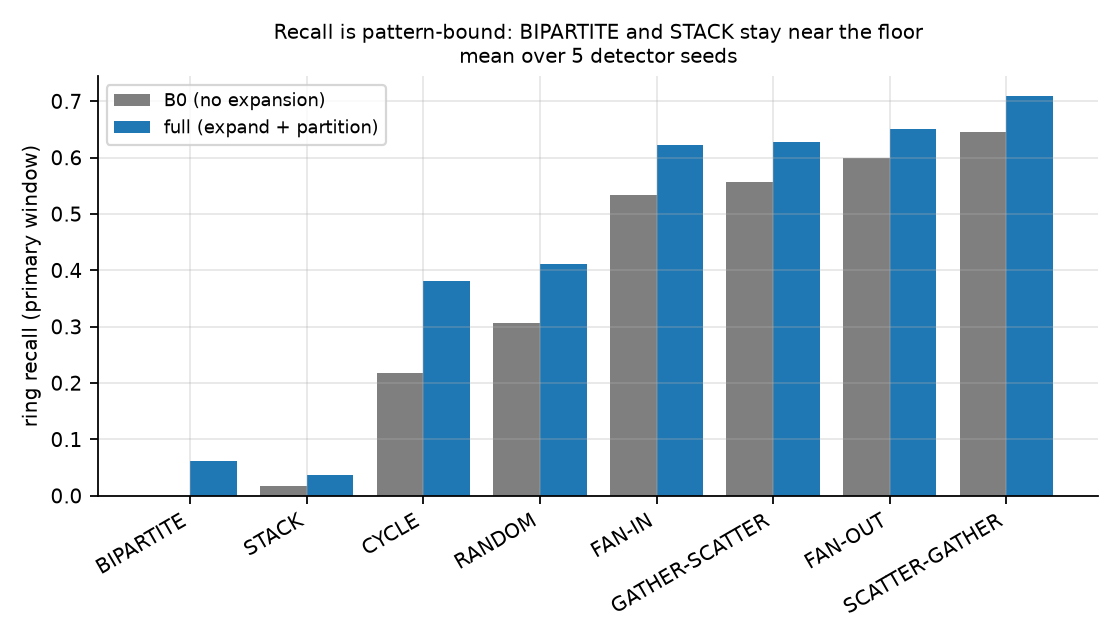
\includegraphics[width=\linewidth]{f2_per_pattern_recall.png}
  \caption{Per-pattern recall.}
  % source: results/figures/f2_per_pattern_recall.png
\end{subfigure}\hfill
\begin{subfigure}[t]{0.48\textwidth}
  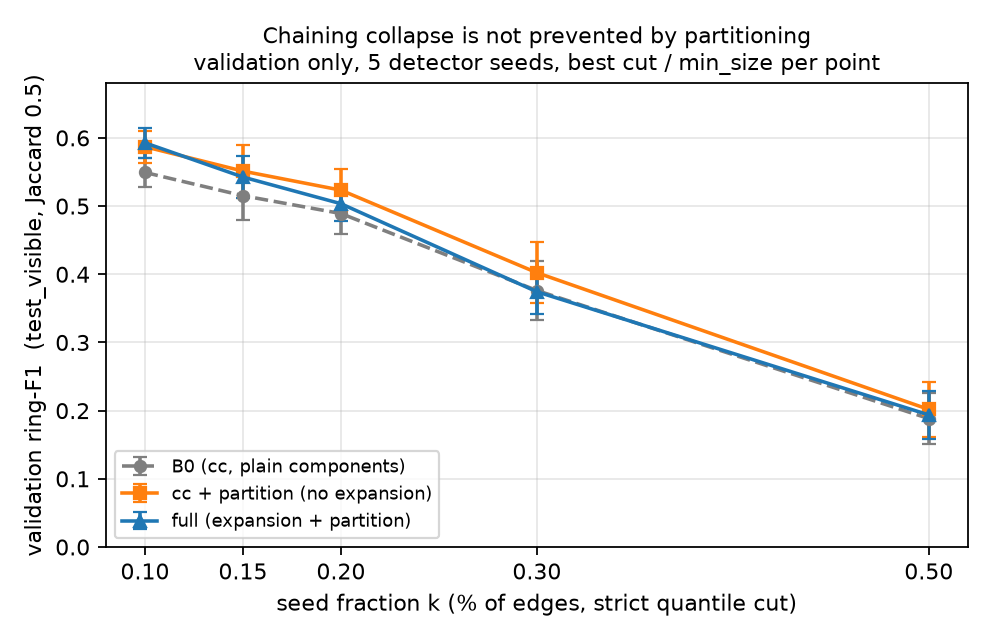
\includegraphics[width=\linewidth]{r4_val_ringf1_vs_seedfrac.png}
  \caption{Validation ring-F1 against seed fraction.}
  % source: results/figures/r4_val_ringf1_vs_seedfrac.png
\end{subfigure}
\caption{Supplementary figures from the repository.}
\label{fig:appendix-figs}
\end{figure}

\section{Corrections made during the project}
\label{app:corrections}

Four claims were corrected before this draft and appear in the paper only in corrected form.
(i) An earlier bound on ring recall derived from \texttt{min\_size} was circular and is
withdrawn (Section~\ref{sec:results-ceiling}). (ii) An earlier, much lower typing accuracy
came from an evaluation lookup that typed a different ring than the matched one; it was found
by an independent check from the explanation layer and fixed with a regression test. (iii) The
partially recovered rings were first read as chains the policy declined to follow; the
connectivity measurement shows most missing members were never reachable. (iv) An earlier
comparison suggested a per-account seed budget lowers baseline ring-F1; at an equal budget it
does not.
% source: docs/FINDINGS.md (B7/B9, B10, B12/B13, and the dated correction to B14)

\section{System context: explanations and platform}
\label{app:platform}

The rings feed two components that are delivered capabilities, not validated research claims.
Their numbers come from their own reports and are outside the findings file this paper is
otherwise restricted to.
% source: docs/FINDINGS.md (scope note of 2026-11-12); README.md

\paragraph{Explanations.}
Each ring receives transaction weights (calibrated score and flow share), account roles,
TreeSHAP feature attributions and a fixed-template narrative; there is no language model.
Median latency is 393\,ms per ring. On the standard fidelity metric the ranking is
indistinguishable from score-only because most matched rings contain only true transactions;
on the 52 instances that mix true and false transactions, score-only is better than the mixed
ranking ($+0.058$ [$+0.010$, $+0.133$]). An internal three-person review of 30 explanations
found the named accounts right at a 0.91 yes-rate and the stated shape plausible at 0.53; it
was not an analyst study, and an external one is designed but not run.
% source: explainability/report/xai_chapter.md §5.2, §7; docs/deep-analysis.md §11, §14

\paragraph{Platform.}
A multi-bank analyst dashboard serves the rings with per-bank isolation enforced by database
row-level security, records verdicts, and gates retraining on a frozen holdout
(Figure~\ref{fig:platform}).
% source: docs/report.md §3.1–3.2
A pooled model applied to one bank's view recovers \ci{0.088}{0.031}{0.161} of tenant-ring
pairs against \ci{0.359}{0.239}{0.500} with the pooled view (Table~\ref{tab:r10}); 172 of 174
rings span more than one bank. Pooling the five studied banks closes 11\,\% of that gap
(0.121 to 0.147).
% source: results/tables/r10_registered.json; results/tables/r10_consortium.json; docs/report.md §7.2
A drift-monitoring experiment could not be made testable on the two-day primary window: the
detector's scores have a tie plateau across the 99th percentile, and day 9 already differs
from day 8 by more than the synthetic shift.
% source: docs/R12.md (second registration); results/platform/r12b/summary.json

% Source: results/tables/r10_registered.md / r10_registered.json, as summarised in docs/report.md §7.2
% R10 is a platform-side experiment registered in docs/TENANT_SIZES.md; it is NOT in docs/FINDINGS.md.
\begin{table}[t]
\centering
\caption{Ring recall of a pooled model applied to one
bank's view vs.\ the pooled view. Banks 1, 20, 11, 118, 12; 68 tenant-ring pairs; 10{,}000
bootstrap resamples. The gap includes distribution shift, so it is not only the cost of seeing
fewer edges.}
\label{tab:r10}
\small
\begin{tabular}{lccc}
\toprule
Row & Bank alone & Pooled & Pooled $-$ bank \\
\midrule
Primary: bank's own scores, features, embeddings & \ci{0.088}{0.031}{0.161} & \ci{0.359}{0.239}{0.500} & \ci{0.271}{0.154}{0.407} \\ % source: r10_registered.json (rows.primary); docs/report.md §7.2
Pooled scores on the bank's edges & \ci{0.121}{0.054}{0.205} & 0.359 & \ci{0.238}{0.135}{0.363} \\ % source: docs/report.md §7.2 (R10 table)
Matched seed budget & \ci{0.076}{0.020}{0.151} & 0.359 & \ci{0.282}{0.167}{0.417} \\ % source: docs/report.md §7.2 (R10 table)
\bottomrule
\end{tabular}
\end{table}


\begin{figure}[t]
\centering
\begin{subfigure}[t]{0.48\textwidth}
  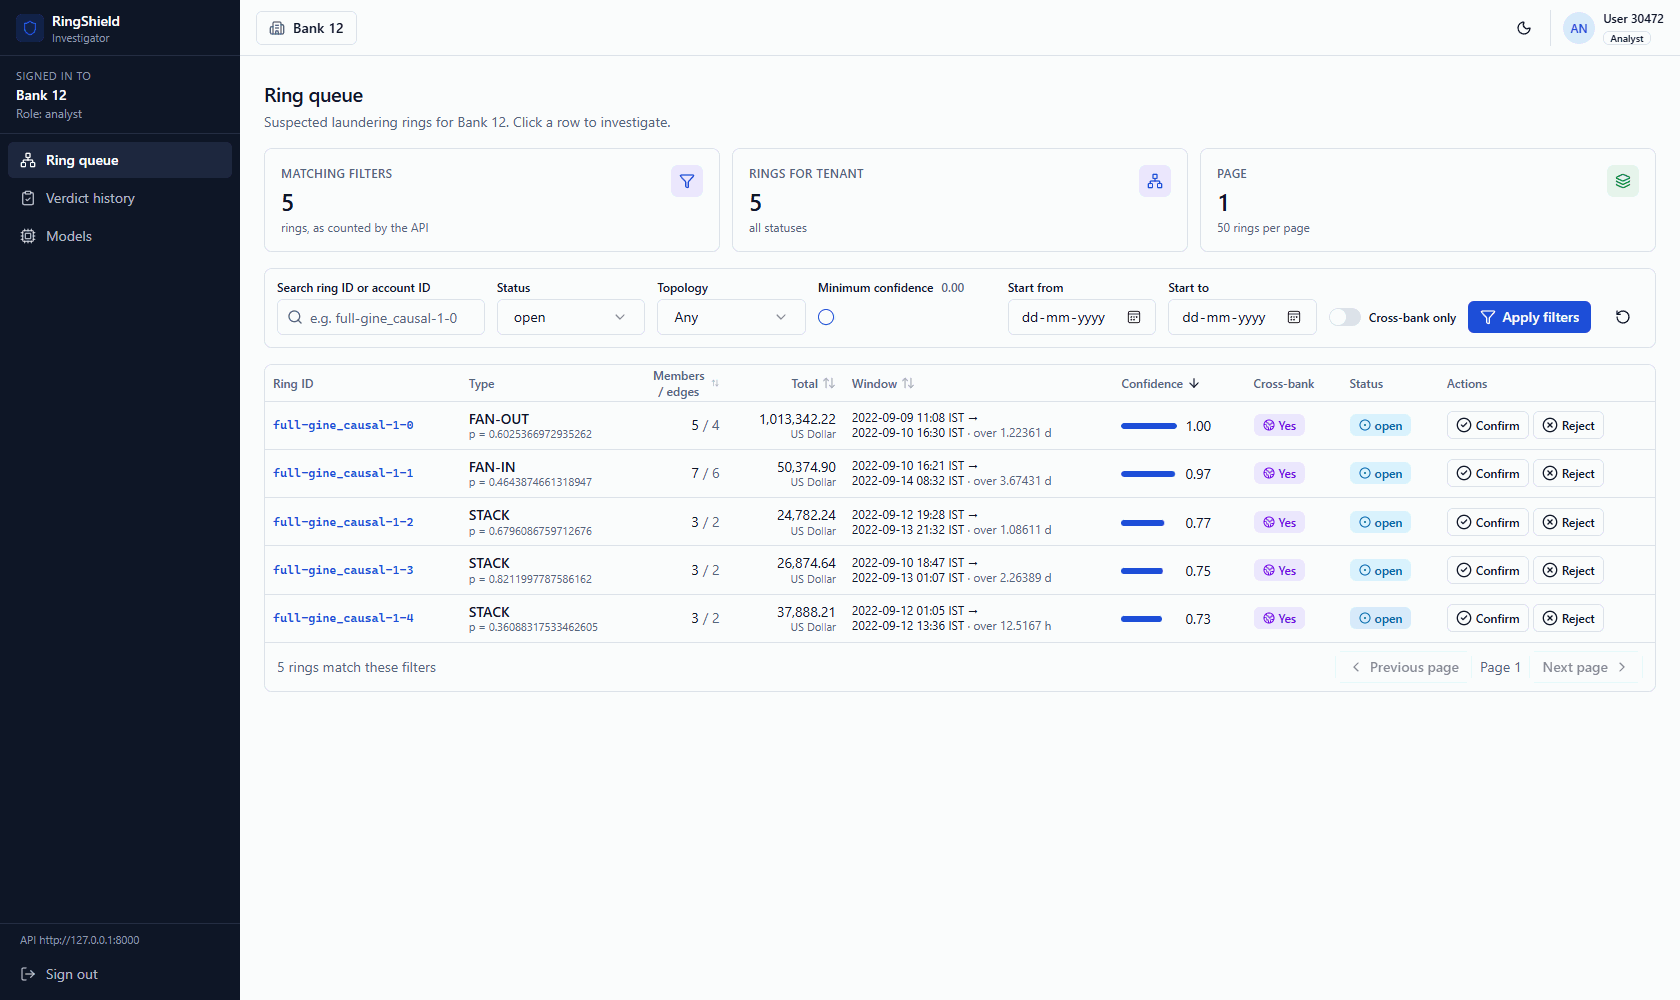
\includegraphics[width=\linewidth]{02-ring-queue-light.png}
  \caption{The analyst's ring queue.}
  % source: docs/screenshots/02-ring-queue-light.png
\end{subfigure}\hfill
\begin{subfigure}[t]{0.48\textwidth}
  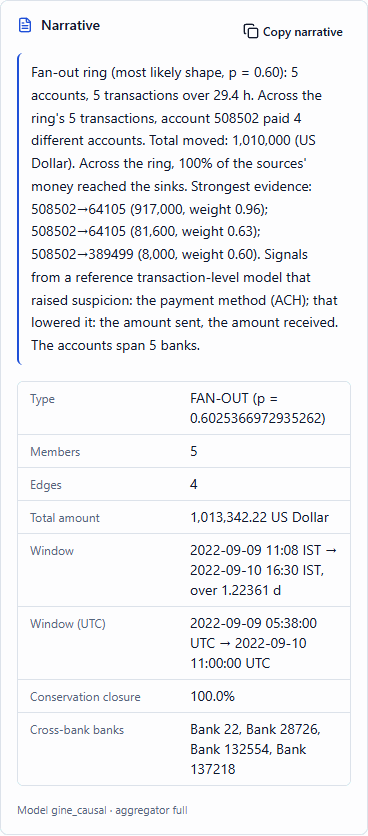
\includegraphics[width=\linewidth]{05-ring-detail-narrative-light.png}
  \caption{A ring's narrative.}
  % source: docs/screenshots/05-ring-detail-narrative-light.png
\end{subfigure}
\caption{The multi-bank analyst platform.}
\label{fig:platform}
\end{figure}


\end{document}
